\documentclass[]{acmsig-alternate-10pt}

% The following \documentclass options may be useful:
%
% 10pt          To set in 10-point type instead of 9-point.
% 11pt          To set in 11-point type instead of 9-point.
% authoryear    To obtain author/year citation style instead of numeric.

\usepackage{amsmath}
\usepackage{graphicx}
\usepackage{url}
\usepackage{amssymb}
\usepackage{subfigure}
\usepackage{algorithm} 
\usepackage{algpseudocode}
\usepackage{epsfig}
%\usepackage{times}

% make an environment for subfigures with verbatim
\newbox\subfigbox	% Create a box to hold the subfigure. 
\makeatletter
  \newenvironment{subfloat}% % Create the new environment. 
    {\def\caption##1{\gdef\subcapsave{\relax##1}}%
    \let\subcapsave=\@empty % Save the subcaption text.  
    \let\sf@oldlabel=\label 
    \def\label##1{\xdef\sublabsave{\noexpand\label{##1}}}%
    \let\sublabsave\relax  %
    \setbox\subfigbox\hbox 
        \bgroup}% 
     {\egroup   %
    \let\label=\sf@oldlabel
    \subfigure[\subcapsave]{\box\subfigbox}}% 
\makeatother

\newcommand{\eightpoint}{\fontsize{8pt}{10pt}\selectfont}
\newcommand{\ninepoint}{\fontsize{9pt}{11pt}\selectfont}

%\advance \baselineskip by 0.4pt

% do not indent paragraphs of enumerated lists (my lists go on for pages...)
% numbers flush left to paragraph text: \leftmargin=17pt
\newcommand{\mybegin}{\begin{list}{\labelenumi}{\leftmargin=\parindent}\usecounter{enumi}}
\newcommand{\myitem}[1]{\item {\textit{\textbf{#1}}}}
%\newcommand{\myitem}[1]{\item {\bf #1}}
\newcommand{\myend}{\end{list}}
\newcommand{\mt}[1]{\mbox{\it #1}}
\newcommand{\todo}[1]{\framebox {\bf #1}}

\begin{document}

%\conferenceinfo{PLDI  2011}{June 2011, San Jose, CA.} 
%\copyrightyear{2010} 
%\copyrightdata{[to be supplied]} 

%\titlebanner{banner above paper title}        % These are ignored unless
%\preprintfooter{short description of paper}   % 'preprint' option specified.

\title{Representing and Parallelizing Induction Variable State in Stream Programs}

%\author{}
%           {}
%            {}
% \authorinfo{Name2\and Name3}
%            {Affiliation2/3}
%            {Email2/3}

\maketitle
\begin{abstract}
As DSP programming is becoming more complex, there is an increasing
need for high-level abstractions that can be efficiently compiled.
Toward this end, we present a set of aggressive optimizations that
target linear sections of a stream program.  Our input language is
StreamIt, which represents programs as a hierarchical graph of
autonomous filters.  A filter is linear if each of its outputs can be
represented as an affine combination of its inputs.  Linear filters
are common in DSP applications; examples include FIR filters,
expanders, compressors, FFTs and DCTs.

We present a linear extraction analysis that automatically detects
linear filters based on the C-like code in their {\tt work} function.
Once linear filters are identified, we show how neighboring nodes can
be collapsed into a single linear representation, thereby eliminating
many redundant computations.  Also, we describe a method for
automatically translating linear nodes into the frequency domain,
thereby yielding algorithmic savings for convolutional filters.

We have completed a fully-automatic implementation of the above
techniques as part of the StreamIt compiler, and we demonstrate
performance improvements that average 400\% over our benchmark
applications.




\end{abstract}

%\category{CR-number}{subcategory}{third-level}

%\terms
%term1, term2

%\keywords
%keyword1, keyword2

\section{Introduction}

Applications that are structured around some notion of a ``stream''
are becoming increasingly important and widespread.  There is evidence
that streaming media applications are already consuming most of the
cycles on consumer machines \cite{Rix98}, and their use is continuing
to grow.  In the embedded domain, applications for hand-held
computers, cell phones, and DSP's are centered around a stream of
voice or video data.  The stream abstraction is also fundamental to
high-performance applications such as intelligent software routers,
cell phone base stations, and HDTV editing consoles.

Despite the prevalence of these applications, there is surprisingly
little language and compiler support for practical, large-scale stream
programming.  Of course, the notion of a stream as a programming
abstraction has been around for decades \cite{SICP}, and a number of
special-purpose stream languages have been designed (see
\cite{survey97} for a review).  Many of these languages and
representations are elegant and theoretically sound, but they often
lack features and are too inflexible to support straightforward
development of modern stream applications, or their implementations
are too inefficient to use in practice.  Consequently, most
programmers turn to general-purpose languages such as C or C++ to
implement stream programs.

There are two reasons that general-purpose languages are inadequate for
stream programming.  Firstly, they are a mismatch for the application
domain.  That is, they do not provide a natural or intuitive
representation of streams, thereby having a negative effect on
readability, robustness, and programmer productivity.  Moreover, because
the widespread parallelism and regular communication patterns of data
streams are left implicit in general-purpose languages, compilers are
not stream-conscious and do not perform stream-specific optimizations.
As a result, performance-critical loops are often hand-coded in a
low-level assembly language and must be re-implemented for each target
architecture.  This practice is labor-intensive, error-prone, and very
costly.

Secondly, general-purpose languages are a mismatch for the emerging
class of grid-based architectures \cite{smartmemories,rawshort,trips} that
are especially well-suited for stream processing.  Perhaps the primary
appeal of C is that it provides a ``common machine language'' for
von-Neumann architectures.  That is, it abstracts away the
idiosyncratic differences between machines, but encapsulates their
common properties: a single program counter, arithmetic operations,
and a monolithic memory.  However, for grid-based architectures, the
von-Neumann model no longer holds, as there are multiple instruction
streams and distributed memory banks.  Thus, C no longer serves as a
common machine language--in fact, it provides the wrong abstraction
for the underlying hardware, and architecture-specific directives are
often needed to obtain reasonable performance.  Again, this greatly
complicates the job of the programmer and hampers portability.

StreamIt is a language and compiler specifically designed for modern
stream programming.  The StreamIt language has two goals: first, to
provide high-level stream abstractions that improve programmer
productivity and program robustness within the streaming domain, and
second, to serve as a common machine language for grid-based
processors.  At the same time, the StreamIt compiler aims to perform
stream-specific optimizations to achieve the performance of an expert
programmer.

This paper motivates, describes, and justifies the high-level language
features of StreamIt, version 1.0.  The major limitation of StreamIt
1.0 is that all flow rates in the streams must be static; applications
such as compression that have dynamically varying flow rates will be
the subject of future work.  A large set of applications can be
implemented with static rates, and while dynamic rates will require a
different runtime model, it will still be essential to fully analyse
and optimize static sub-sections in order to obtain high performance.

The paper is organized as follows. In Section {\ref{sec:domain}}, we
characterize the domain of streaming programs that motivates the
design of StreamIt, and in Section~\ref{sec:overview} we describe the
language features in detail.  We present an in-depth example of a
software radio in Section~\ref{sec:example}, preliminary results in
Section~\ref{sec:results}, related work in Section~\ref{sec:related},
and conclusions in Section~\ref{sec:conc}.


%\begin{figure}[t]
%\eightpoint
%\begin{Verbatim}[numbers = left]
%int->int filter AssignPictureType(int width, 
%        int height, 
%        int numpictures) {
%    int frameno;
%
%    init {
%        frameno = 0;
%    }
%
%    work pop (width*height*3) push 2 {
%        push(frameno);
%        for (int i = 0; i < width*height*3; i++) {
%            pop();
%        }
%
%        int pushval;
%        int framecount = frameno % 12;
%        if (framecount == 0) {
%            pushval = 1;
%        } else if (framecount == 3 
%                || framecount == 6 
%                || framecount == 9) {
%            pushval = 2;
%        } else {
%            pushval = 3;
%        }
%
%        if ((frameno == (numpictures-1)) 
%            && (pushval == 3)) {
%            pushval = 2;
%        }
%
%        push(pushval);
%        frameno++;
%    }
%}
%\end{Verbatim}
%
%\caption{Example StreamIt program with AssignPictureType filter, used in MPEG Encoder.\protect\label{fig:apt-pipeline}}
%\end{figure}

\section{The StreamIt Language}
\label{sec:streamit}

StreamIt is an architecture-independent language for high-performance
stream programming~\cite{thies-cc02}.  The compiler is publicly
available~\cite{streamitweb} and includes backends for multicore
architectures, clusters of workstations, and Tilera architectures.

The model of computation in StreamIt is grounded in (but not limited
to) synchronous dataflow~\cite{lee87}.  In this model, the programmer
implements independent actors, or {\it filters}, which translate data
items from input channels to output channels.  Filters are composed
into graphs that represent the overall computation.  The key property
of synchronous dataflow is that the number of items consumed and
produced during each execution of a filter is known at compile time,
allowing the compiler to perform static scheduling and optimization.

An example StreamIt filter appears in Figure~\ref{fig:apt-pipeline}.
It is based on the AssignPictureType filter in the MPEG2 encoder.
StreamIt filters contain three stages of execution.  The most
important is the \work function, which represents the
steady-state execution step and is called repeatedly by the runtime
system.  Within the \work function, a filter may {\it peek} at a given
element on the input tape, {\it pop} an item off the input tape, or
{\it push} an item to the output tape.  The total number of items
peeked, popped, and pushed are declared as part of the \work function.
Note that if the peek rate exceeds the pop rate, it represents a
sliding window computation in which some input elements are accessed
across multiple invocations of the filter.

In addition to the \work function, a filter may declare an {\tt init}
function to initialize internal data structures, as well as a 
 \prework function (not given in Figure~\ref{fig:apt-pipeline}) to
perform specialized processing of data items prior to the steady
state.  The \prework function is needed in cases where the initial
processing has a different input or output rate than the steady-state
processing.

A {\it schedule} gives a multiplicity for each filter in a stream
graph.  The multiplicity indicates how often a filter's \work function
should be invoked (or \prework function on the first iteration of the filter).  The
{\it steady-state schedule} can be calculated such that all filters
fire in the schedule, and the schedule can be repeated
indefinitely~\cite{lee87}.  Steady-state execution of the graph
entails repeating the steady-state schedule for as much input as is
expected.  Execution of the stream graph is conceptually wrapped in an
outer loop that continuously executes the steady-state schedule.  All
the multiplicities of the steady-state can be multiplied by the same
constant $m$, and the result will still be a valid steady-state.  We
call this process {\it increasing} the steady-state of the graph by
$m$.

Furthermore, an {\it initialization} schedule enables the steady-state
schedule in the presence of peeking filters.  An initialization
schedule is required if peeking is present in a graph to enable the
calculation and execution of a steady-state
schedule~\cite{karczmarek-lctes03}.  During application execution, the
{\it init} function is called once for each filter, then the
initialization schedule is executed once, followed by an infinite
repetition of the steady-state schedule.

As depicted in Figure~\ref{fig:structures}, StreamIt provides three
hierarchical primitives for composing filters into stream graphs.  A
{\it pipeline} represents a sequential composition of streams, in
which the output of one stream feeds into the input of the next.  A
{\it splitjoin} represents a parallel set of streams, which divulge
from a common {\it splitter} and converge to a common {\it joiner}.
The types of splitters and joiners are predefined by the StreamIt
language; they encompass duplication and weighted round-robin
behaviors.  Finally, a {\it feedbackloop} represents a cycle in the
stream graph.

\begin{figure}[t!]
\centering
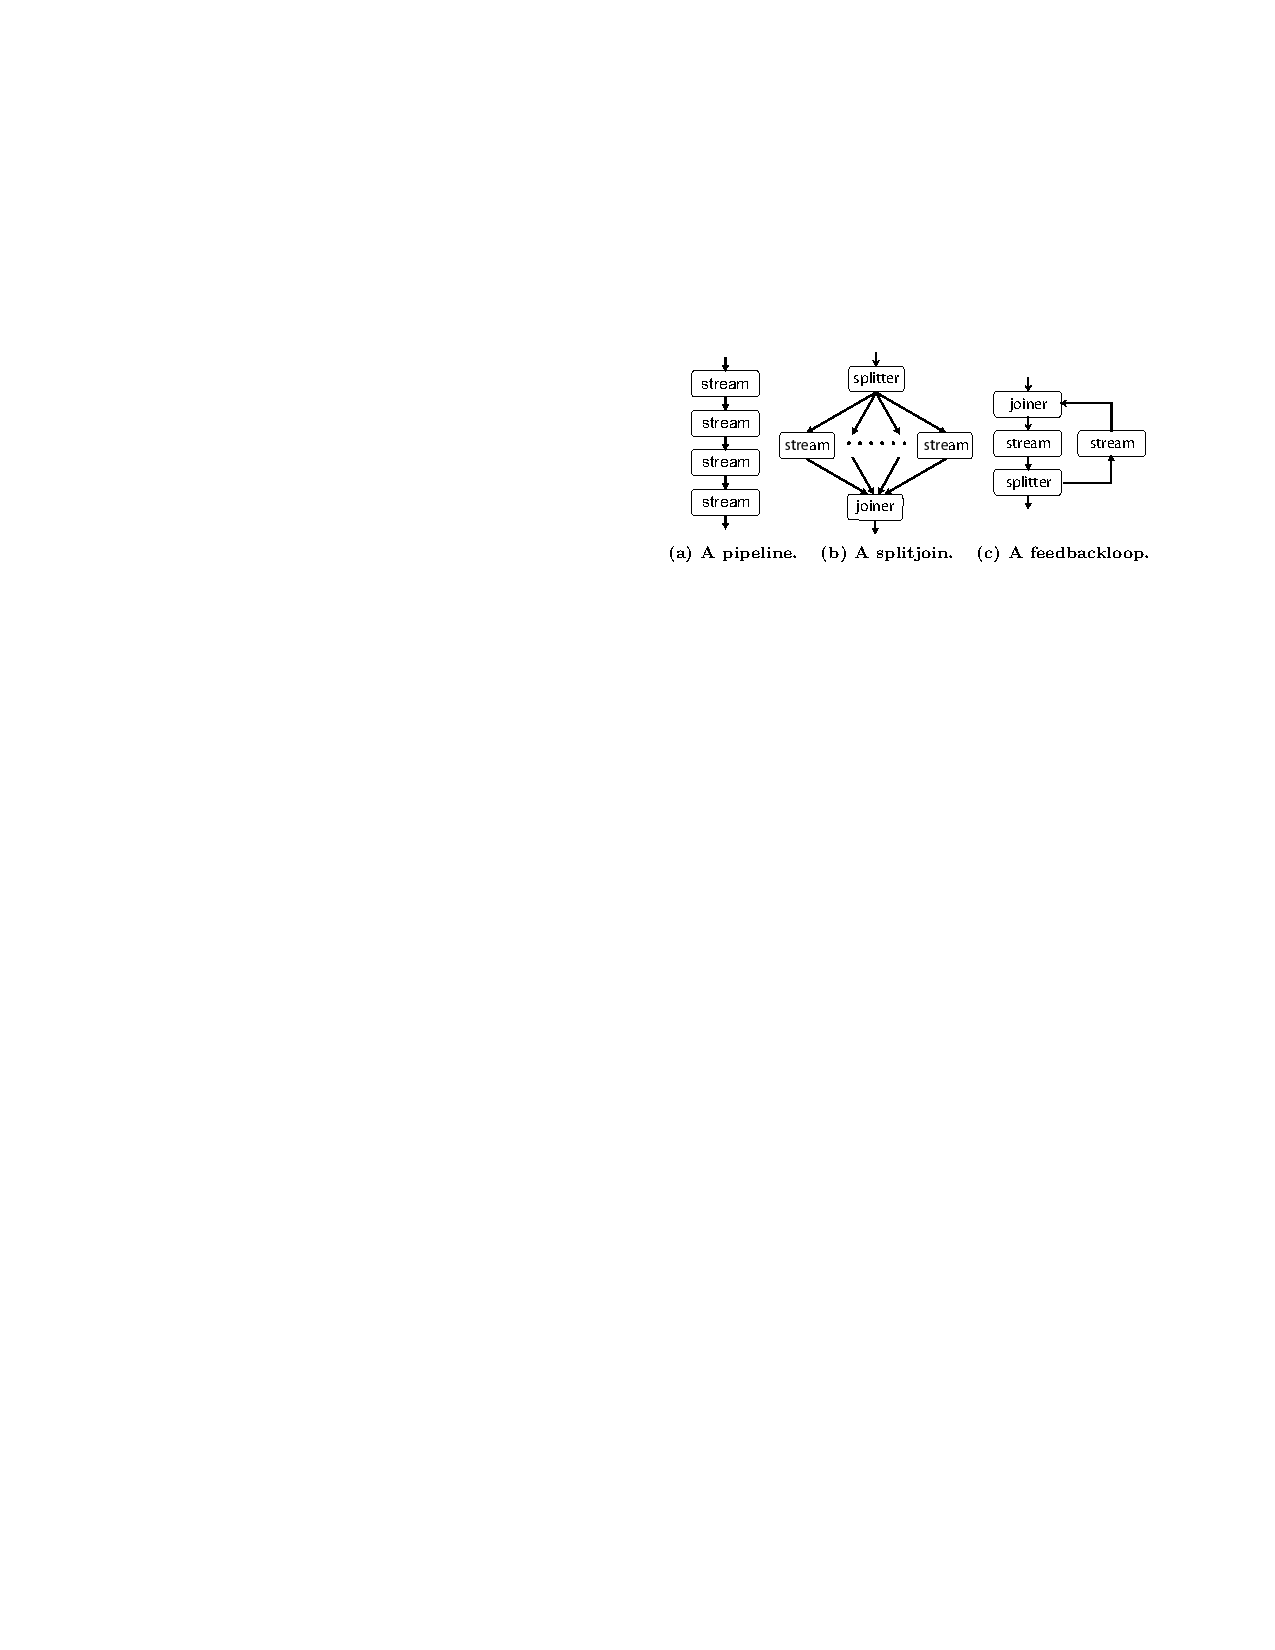
\includegraphics[width=3.3in]{stream-structures.pdf}
%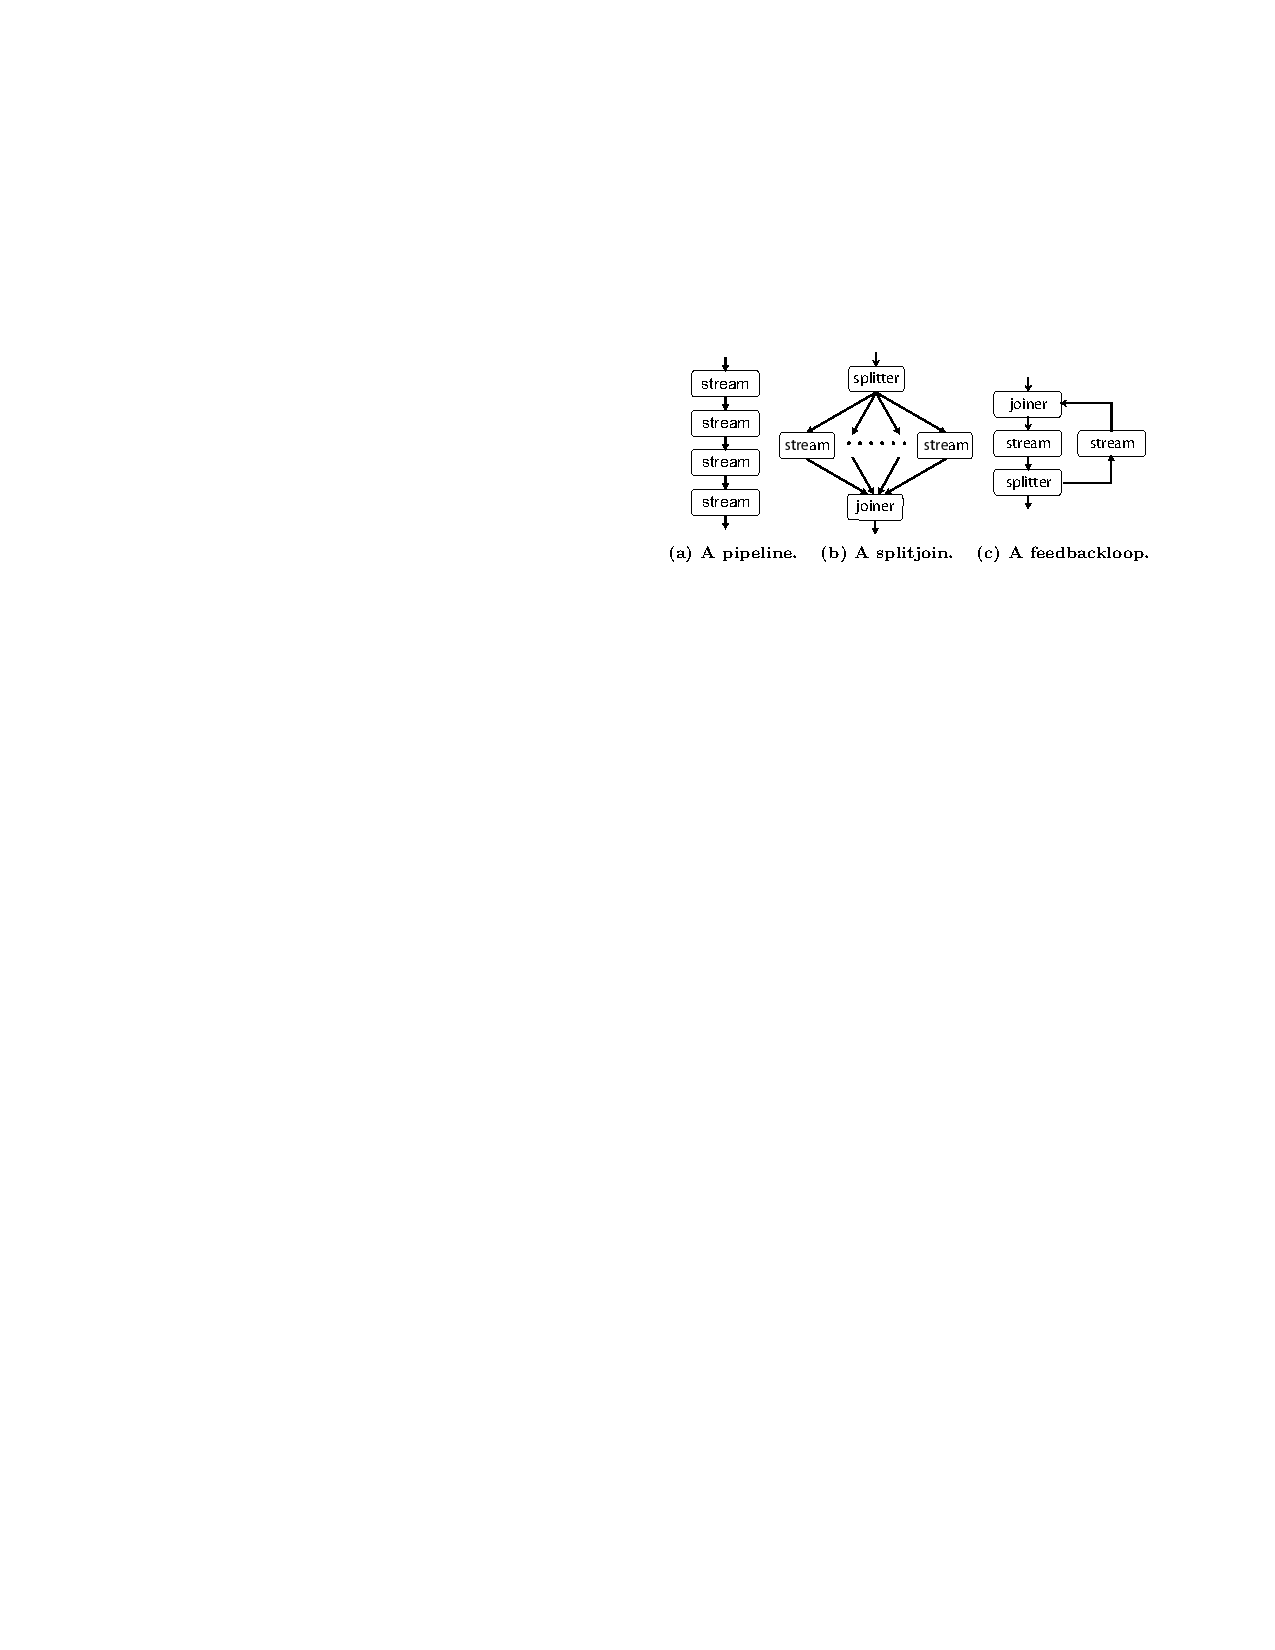
\psfig{file=stream-structures,width=\columnwidth}
\caption{Hierarchical stream structures supported by StreamIt.\protect\label{fig:structures}}
\end{figure}

The StreamIt compiler coarsens the granularity of a stream graph by
applying the {\it fusion} transformation which merges adjacent filters
into a single (large) filter (embedding the schedules of execution in
the merged filter)~\cite{streamit-asplos}.  The {\it fission}
transformation is employed to add data parallelism to a stream graph.
In fission, a single filter without state is duplicated a certain
number of ways and placed in a splitjion construct.  Input items to
the original filter are distributed among the duplicates, termed {\it
  fission products}.  In \S\ref{sec:fission}, we describe how to
extend the fundamental fission transformation to parallelize induction
variable state.

\section{Induction Variable State in Stream Programs}
\label{sec:inductionstate}

% \begin{figure}[t]
% {\eightpoint
% \begin{verbatim}
%   int->int stateful filter InductionFilter() {
%       int counter;
%       int max;
  
%       work push 1 pop 1{

%           ...

%           counter = (counter + 1);

%           if (counter > max) {
%               counter = 0;
%           } 
%       }
%   }
% \end{verbatim}
% \caption{Example of a stateful StreamIt filter using induction variable state.\protect\label{fig:filter-example}}}
% \end{figure}

Traditional induction variables encapsulate all variables that are
increased or decreased with iterations of a loop~\cite{Aho:1986, Fischer:2009}.  Induction variable
state as applied to stream programming is a class of state that
requires keeping count of how often a filter has been invoked.  Common
usage of induction variable state includes performing some special
action after a certain number of iterations and keeping track of array
index positions.  Many filters maintain multiple induction variables
as well, which may either be dependent or independent of each other.

Many applications in the StreamIt benchmark suite, including MPEG2 encoder,
Medium Pulse Doppler, Trellis, and FIRBank (pipelined version), maintain induction variable state 
by creating a mutable state field in the corresponding filter.  This
state can be set to the desired starting value.  The induction
variable is consistently updated at some point during the work call.
For many use cases, this induction variable may need to be reset if it
reaches a certain threshold. 

Figure~\ref{fig:apt-pipeline} illustrates a common pattern of explicit
induction variable state.  It is based on the AssignPictureType filter in 
the MPEG2 encoder. The implementation of the filter maintains
a filter variable {\tt frameno} that is incremented on each call of
the {\tt AssignPictureType}'s work function.  This variable
represents state.  Each iteration of the 
filter uses a value for {\it frameno} dependent on what the value of
{\it frameno} was in the previous iteration.  The {\tt framecount} variable is derived
from this state and used in control flow.

As presently constructed, induction variable state for\-ces the
corresponding filter to be run in sequential order.  In providing a
mutable state whose value is dependent on the previous execution step,
it is necessary to run a filter execution step and establish the
induction variable value before moving on to the next execution step.
The tradition fission transformation would not be able to parallelize
this filter without understanding how to properly distribute the
calculation of the state.  As such, it is not possible 
to create duplicates and run them in a parallel fashion.  

With induction variable state, it is possible to make the 
compiler aware of such state through the keyword solution.  
Figure~\ref{fig:apt-pipeline} shows how the same AssignPictureType filter can be 
rewritten to use the keyword.  The compiler can generate the value
for {\tt iter()} for each iteration of the AssignPictureType filter independent
of previous iterations.  Duplicates of the filter can be made and
data parallelism opportunities can be exploited.


\subsection{Scalability Implications of Eliminating Induction Variable State}
\label{sec:model-analysis}
Table~\ref{fig:benchmarks} indicates programs in the StreamIt benchmark suite that use induction variable filters (not including source filters) in the manner described above.  The StreamIt compiler provides static estimations of work performed in filters.  The above table indicates the work performed in specifically the induction variable filters.

The majority of programs do not have substantial work performed in filters using induction variables; FIRBankPipeline and MPD contain only a few stateful filters whose total work concentration is fairly low.  The MPEG-2 motion estimation subset is the only exception because its stream graph is comprised mostly with stateful filters.  However, eliminating any form of state will have a large impact on runtime performance even on programs with low work concentration in stateful filters.  We model the potential speedups of a particular stateful program in this subsection.  For the purpose of this analysis, we will assume no communication cost between filters.  We will also assume the compiler exposes no pipeline parallelism.  This assumption forces the serialization of stateful filters on the stream graph.

\begin{table}[t]
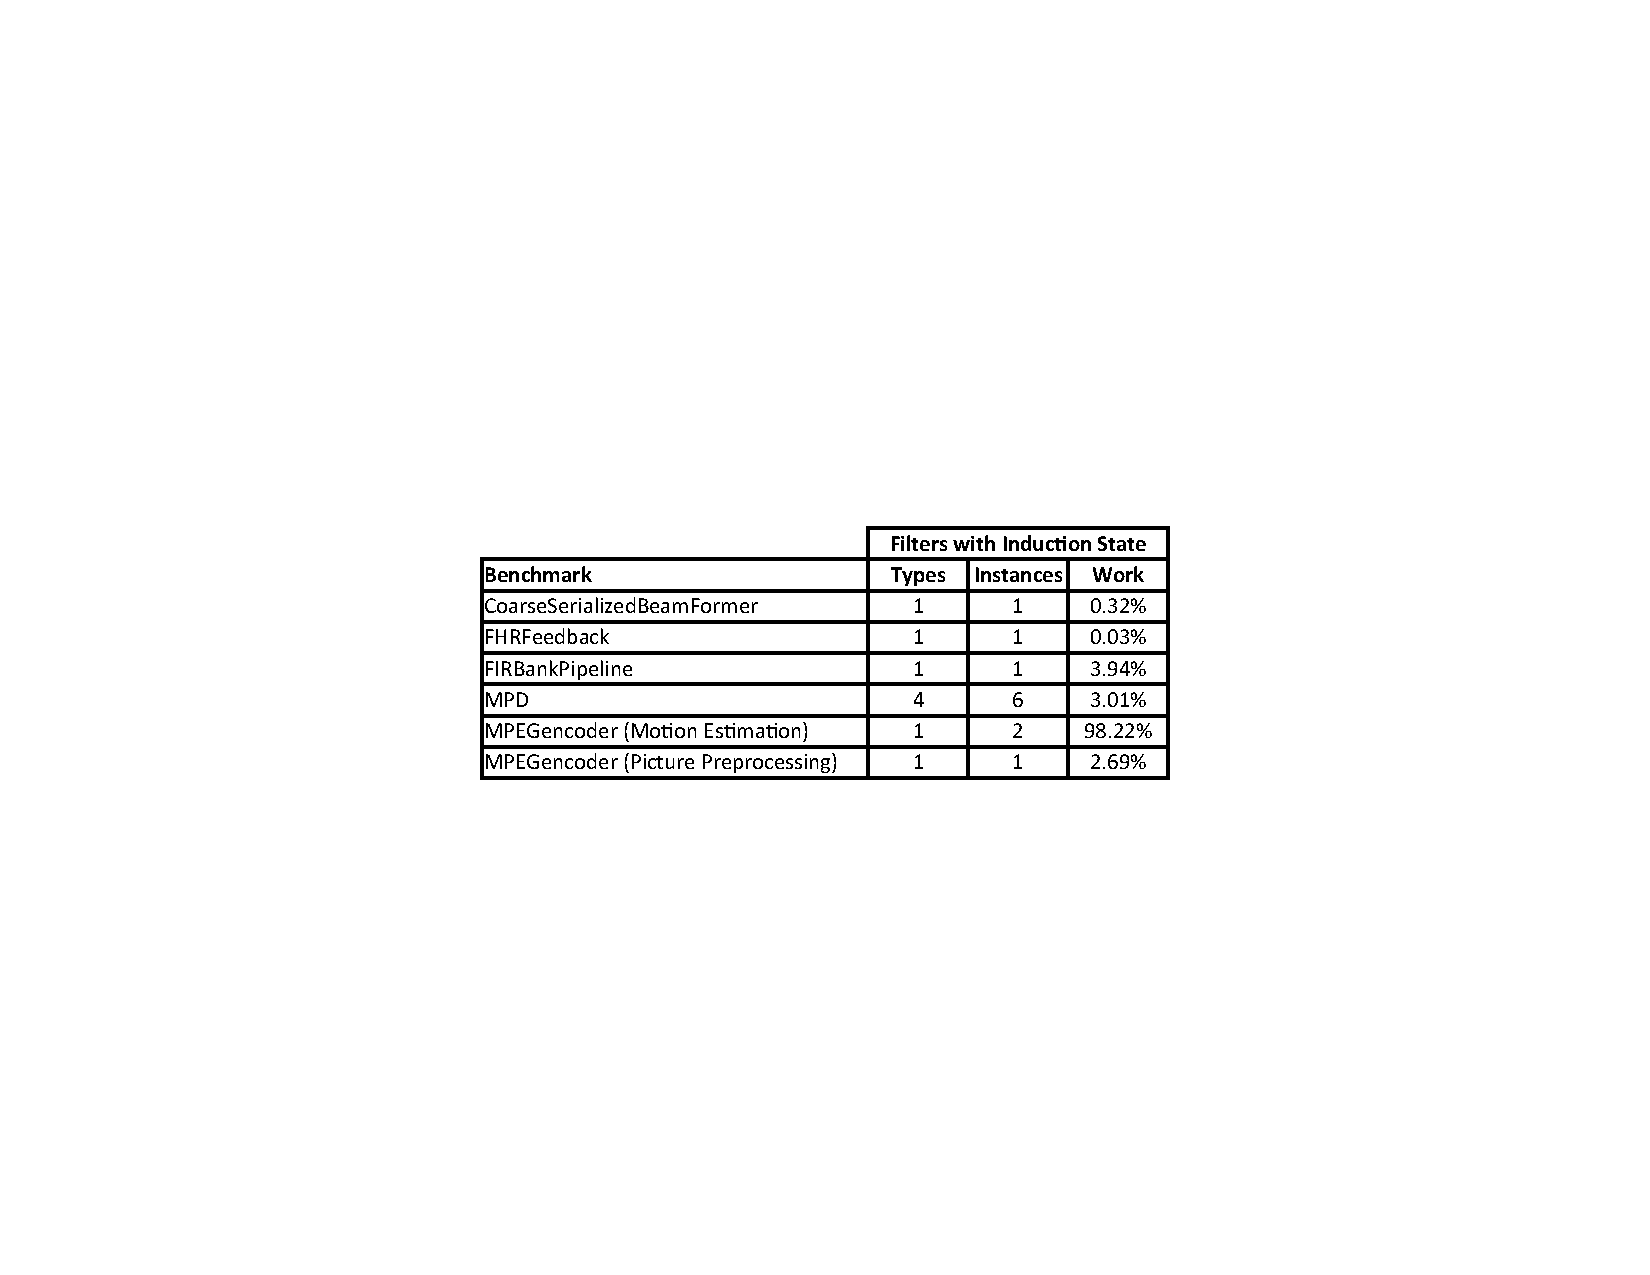
\includegraphics[width=3.3in]{figures/induction-benchmarks.pdf}
\caption{Benchmarks using induction variable state and estimations on work performed in filters with induction state.\protect\label{fig:benchmarks}}
\end{table}

Let $N$ be the number of cores we are planning to parallelize over.  Let $\sigma$ be the percentage of work performed in stateful filters that can have its state eliminated, in this case solely filters that use induction variable state.  

If $\sigma = 0$, the entire program is stateless.  The program can be fused to coarsen the granularity, then fissed and mapped to all of the available cores.  Each core would perform $\frac{1}{N}$ of the total work.  Thus with no state, the program can exhibit speedups of up to $N$ times the single-core runtime.

For filters that contain stateful work, $1-\sigma$ of the work in the program is considered stateless, and thus can be fissed and assigned to $N$ individual cores.  The stateful filters cannot be parallelized, and is sequential to all work in the program.  The total serialized work is $\frac{1-\sigma}{N} + \sigma$.  Thus the total speedup is the serial work divided by the new parallelized work.  
\begin{eqnarray*}
\dfrac{1}{\frac{1-\sigma}{N} + \sigma} &=& \dfrac{N}{1 + \sigma(N-1)}
\end{eqnarray*}

We can characterize the amount of speedup between a completely stateless program to an equivalent stateful program with $\sigma$ percentage of stateful work.  This is simply:
\begin{eqnarray*}
\dfrac{N}{\frac{N}{1 + \sigma(N-1)}} &=& 1 + \sigma(N-1)
\end{eqnarray*}

\begin{figure}[t!]
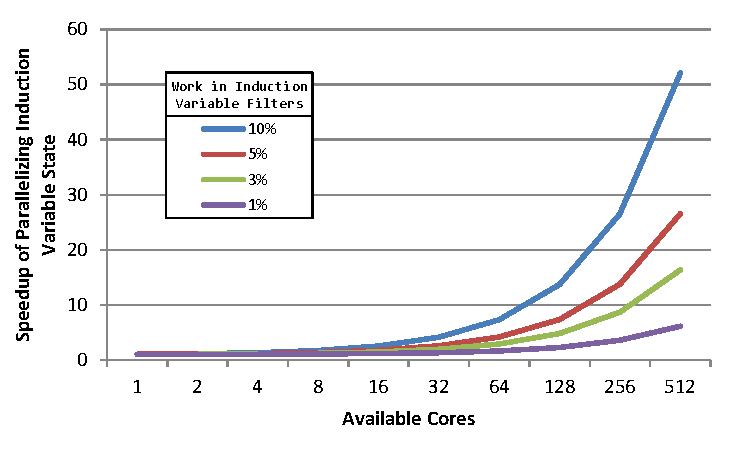
\includegraphics[width=3.3in]{figures/theoretic-speedup.pdf}
\caption{Theoretical speedups of stateless programs over corresponding stateful programs with $\sigma$\% work in filters using induction variable state.  \protect\label{fig:theo-speedups}}
\end{figure}

Figure~\ref{fig:theo-speedups} indicates the potential speedups over stateful programs given stateful work percentages and a varying number of cores.  Even benchmarks in the suite that exhibit only 3\% work in stateful filters can exhibit 8x speedups with 256 cores.  Providing a means to remove state from filters that exhibit very small amounts of work relative to the rest of the program can still generate substantial speedups in the near future.


\section{Design Rationale}

Our approach in removing induction variable state is to introduce a new language construct.  The language construct maintains a value indicating how often the corresponding filter has been invoked.  This approach was chosen over implementing a system to automatically recognize induction variable usage in filter construction.

The approach of automatic analysis would require looking for an induction variable defined in the filter.  The simplest form of this analysis would require first idiomatically detecting for a variable modified by a statement similar to \texttt{var = var + 1}.  Very few iteration filters (outside of source filters) use induction state in this limited capacity.  Consider Figure~\ref{fig:weight-calc}, where the induction variable is incremented at each iteration step, until a certain threshold value at which it will reset.  This pattern is very common in programs that use induction filters.  MPD and FIRBank use this technique to iterate across a provided array one element per iteration step.  To ensure consistency between iteration steps, the automatic analysis is required to detect these types of updates as well.  

\begin{figure}[t]
{\eightpoint
\begin{verbatim}
float->float stateful filter WeightCalc(int n)
{
  float[n] window;
  int windowPos;

  ...

  // the input stream is multiplied with the weights
  work push 2 pop 2
  {

    push(pop() * window[windowPos]);
    push(pop() * window[windowPos]);

    windowPos++;
    if(windowPos >= n)
    {
      windowPos = 0;
    }
  }
}
\end{verbatim}
\caption{MPD filter that multiplies stream values with weights.\protect\label{fig:weight-calc}}}
\end{figure}

\begin{figure}[t]
{\eightpoint
\begin{verbatim}
float->float stateful filter CFARDetectFilter(int rows, int cols)
{
  int currentCol;
  int currentRow;

    ...

  work pop 3 push 1
  {
      ...

    currentRow++;
    if(currentRow >= rows)
    {
      currentRow = 0;

      currentCol++;
      if(currentCol >= cols)
      {
        currentCol = 0;
      }
    }
  }
}
\end{verbatim}
\caption{MPD CFAR Detect filter.\protect\label{fig:cfar-detect-filter}}}
\end{figure}

A filter may have multiple induction variables that are dependent on one another in defining their values.  Consider Figure~\ref{fig:cfar-detect-filter}, a filter used in MPD maintaining nested induction variables.  The automatic analysis must also be able to detect incrementing statements that may not necessarily be updated on every work call.  The process of simply detecting and identifying induction variables can potentially branch into many cases that need to be specially implemented.

There may potentially be other special cases that must be defined into the automatic analysis.  Filters may have also define induction variables to start with and reset to a particular value.  Induction variables may increment by a different value other than 1 at each execution step.  Though the methods of using induction variables as illustrated in Figure~\ref{fig:cfar-detect-filter} and Figure~\ref{fig:weight-calc} encompass many of the common use cases in the benchmark suite, slight variations in the implementation to the pattern may prevent the induction variable from being detected.

Accordingly, there are several downsides to the approach of automatic analysis.  Automatic recognition is a fairly inflexible process in detecting induction variable state.  As illustrated, there may be many different ways of defining induction variables.  Nested counters are often used to track row and column indexes in two-dimensional arrays.  Co-induction variables may be constructed to reset the value of other variables after reaching a certain value.  The many different uses of induction variables may be difficult to assess.  Automatic recognition would restrict data parallelism opportunities to only the filters that fit the implemented templates.  We instead elect to provide the user with the flexibility of defining derived induction values while providing parallelism opportunities.  

The keyword solution also has the added benefit of maintaining a value that is predictable in its updates.  The value that the keyword returns is simply the current iteration number for that the corresponding filter has run.  This is a value that always increments by one at the end of every work call.  Automatic recognition is a frail process because it is difficult to predict how the induction value will be updated, as illustrated in the above figures.  

The approach of automatic analysis also does little to encourage programming with parallelism in mind.  User written code will still maintain state, which inhibits data parallelism opportunities.  In introducing a language construct, user written code eliminates explicitly kept state.  This approach encourages users to write code with the intention of exploiting parallelism.



\section{Iteration Keyword}

The stream programming paradigm allows the burden of induction variable state to be shifted from the programmer to the compiler.  With the introduction of a new language construct, hereafter referred to as {\tt iter()}, the programmer can take measures to write their programs with data parallelism in mind.  Use of {\tt iter()} potentially provides further benefits in programmability and code readability as well.

As described before, induction variable state requires the user to maintain mutable state, updating such state within the filter invocation, and potentially resetting them when required.  In providing the {\tt iter()} keyword, the programmer can eliminate much of this code simply by arithmetically manipulating {\tt iter()} usage.  

[examples for single induction variable elimination, multiple nested induction variable elimination, varying starting values]

The transformation from filters using induction variable state to using {\tt iter()} is fairly simple for users to implement.  Many of these transformations follow the same approach as induction variable elimination.  The induction variable can be expressed as an arithmetic manipulation of {\tt iter()}.

In having the user define their induction variables using {\tt iter()}, it is possible to eliminate code required to reset or update the induction value.  For large filters, the maintenance of this state may be difficult to follow.  The approach illustrated in the examples shows how it is possible to remove much of the code required to maintain this state with the {\tt iter()} keyword.  

For filters that define multiple induction variables, it is possible to redefine these values in terms of {\tt iter()} as well.  It is not necessary to maintain multiple separate values for state.  Independent and nested induction variable state alike can be defined with use of {\tt iter()}.

This approach of using {\tt iter} to define induction variable state helps users to write filters in a stateless manner.  The user can think about programming their filters in a stateless manner, and thereby exposing data parallelism. 



\subsection{Comparison to Coarsening}
\label{sec:coarsen}

% \begin{figure}[t]
% {\eightpoint
% \begin{verbatim}
% float->float stateful filter WeightCalc(int n)
% {
%   float[n] window;
%   int windowPos;

%   ...

%   // the input stream is multiplied with the weights
%   work push 2 pop 2
%   {

%     push(pop() * window[windowPos]);
%     push(pop() * window[windowPos]);

%     windowPos++;
%     if(windowPos >= n)
%     {
%       windowPos = 0;
%     }
%   }
% }
% \end{verbatim}
% \caption{MPD filter that multiplies stream values with weights.\protect\label{fig:weight-calc}}}
% \end{figure}

In cases of explicit induction variable state where the induction
variable is reset after a certain number of iterations, the filter can
be converted into a stateless filter by {\it coarsening} the filter,
increasing the number of input items that are required for the work
function execution.  Figure~\ref{fig:wc-example}(a) lists the weight
calculation filter from the Medium Pulse Doppler (MPD) benchmark.  The
filter includes explicit induction variable state as originally
implemented by the programmer.  This filter can be rewritten without
state (and without using the {\tt iter()} keyword) by coarsening the
filter such that each work function execution operates on a larger
subset of the input.  Figure~\ref{fig:wc-example}(b) lists a coarsened
implementation that is stateless.  In the coarsened implementation the
filter requires $2n$ input items.

Figure~\ref{fig:wc-example}(c) lists the implementation of the weights
calculation filter utilizing the {\tt iter()} keyword.  Notice that
the filter operates at a finer granularity versus the coarsened
version and that it operates at the same granularity as the original
filter.  Although the {\tt iter()} implementation includes a modulo
operation per output, calculation of outputs will be parallelized
(see Section~\ref{sec:fission}).

The mantra of stream programming is that the programmer should not be
burdened with parallelization, granularity, communication or
synchronization concerns.  Implementing a filter at a fine granularity
allows the compiler or runtime to decide on the best granularity for a
given architectural target.  In practice the use of the {\tt iter()}
keyword is preferred over a coarsening conversion because:

\begin{itemize}

\item The programmer grasped the algorithm and implemented the
  application at the fine granularity.  A language should constrain
  the programmer as little as possible for the sake of performance.

\item The coarse granularity implementation requires larger input and
output buffers to implement because of the larger push and pop rates.
Larger buffers occupy more of the cache and could evict filter data or
instructions are needed during execution.  Thus there could be more
accesses to longer latency memory hierarchies~\cite{sermulins-lctes05}.

\item Larger input and output rates also interact with the
  steady-state scheduling algorithm.  Since the scheduling algorithm
  is performing many cascading LCMs, a single filter with large input
  and output rates will increase the multiplies of all filters of the
  application, requiring more buffering and increasing
  latency~\cite{karczmarek-lctes03}.  The use of the {\tt iter()}
  keyword does not force the programmer to sacrifice latency for
  parallelization.

\end{itemize}


\section{Desugaring}
\label{sec:desugar}

%\begin{figure}[t]
%{\eightpoint
%\begin{verbatim}
%  int->int filter IterationFilter() {
%
%      work push 1 pop 1{
%
%          int counter = iter();
%          ...
%
%      }
%  }
%\end{verbatim}
%\caption{Example of a StreamIt filter using the iteration keyword.\protect\label{fig:iter-filter-example}}}
%\end{figure}
%
%
%\begin{figure}[t]
%{\eightpoint	
%\begin{verbatim}
%  int->int filter IterationFilter() {
%
%      int __iterationCount = 0;      
%
%      work push 1 pop 1{
%
%          int counter = __iterationCount;
%          ...
%
%          __iterationCount++;
%
%      }
%  }
%\end{verbatim}
%\caption{Example of a StreamIt filter with the iteration keyword desugared.\protect\label{fig:desugar-filter-example}}}
%\end{figure}

%
%\begin{figure}[t!]
%\centering
%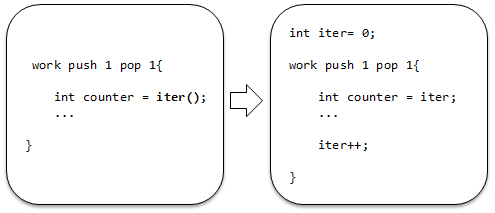
\includegraphics[width=3.3in]{figures/desugaring.png}
%\caption{Desugaring a filter using \texttt{iter()} keyword.\protect\label{fig:desugar}}
%\end{figure}


Under the StreamIt framework, filters are classified as iteration filters when there is use of the iteration keyword in its work function.  A simple lexer and parser can identify the use of this keyword, and it is represented accordingly in the intermediate representation.  To have it actually return the correct iteration value, we first convert the keyword to a compiler-usable construct.

{\tt iter()} is replaced with an access to a field holding the value of the iteration count.  The filter is given a definition for this field only if an {\tt iter()} use exists in its work or prework definition.  The work and prework function are appended with incrementing statements that update the iteration value.

The introduction of this iteration field creates state in the provided filter.  For future operations, the compiler does not consider this iteration field as part of the state of filter.  Future processes will maintain this inherent state without the downsides of introducing state.

It is important to note, these filters are not classified as stateful to the user, even though the filter is actually stateful on the iteration count after the desugaring process.  In classifying filters as stateful, the user is made aware of where data parallelism may be inhibited.  Iteration filters will not inhibit data parallelism because its state is identifiable to the compiler during the fission process.   


\section{Generalized Fission of Sliding Window Filters}
\label{sec:fission}

This section provides an overview of our technique for the fission of
sliding window filters. A complete description is given in
Figure~\ref{fig:general-fission} in the Appendix.  Our technique for
filter fission employs an optimization termed {\it synchronization
  removal}.  This transformation is applied to nodes calculating the
identity function in the general graph such that they can be removed,
but their communication patterns remain embedded in the general
graph. A description of synchronization removal is beyond the scope of
this paper, for a complete exposition, please see~\cite{mgordon-phd}.

The fission transformation applied to $f$ by factor $P$ divides $f$'s
work among $P$ fission products: $f_1...f_P$.  After the
transformation, each $f$ performs $M(S,f) /P$ iterations of $f$'s work
function in the steady-state.  The work of $f$ in the initialization
stage is preserved and translated to $f_1$.  The following
preconditions must be met before it $f$ can be fissed by $P$:
\begin{enumerate}
\item Fission products divide the work of $f$ evenly:
{\ninepoint
\begin{equation}
M(S,f) \mod P = 0 
\label{eq:mod-fiss}
\end{equation}
}
\item The items remaining in the input buffer of the original filter
  after initialization must be less than the number of items that will
  be dequeued by each fission product:
{\ninepoint
\begin{equation}
C(f) < (M(S,f) / P) \cdot o(W, f)
\label{eq:fiss-precond1}
\end{equation}
}
\end{enumerate}

\noindent The second precondition assures that no item is read by more
than 2 fission products.  As Section~\ref{sec:data-par} describes,
both of these preconditions can be enforced on any filter by
increasing the steady-state of the graph.  Fission includes the
following steps: 
\begin{enumerate}
\item Create $P$ copies of $f$ and set their rates
and work functions according to Figure~\ref{fig:general-fission}.
\item Create two identity nodes, $ID_I$ and $ID_O$, that will encode
  the distribution for the fission.
\item Move the initialization stage computation of $f$ to $f_1$
  according to Figure~\ref{fig:general-fission}. 
\item Move input distribution of $f$ to $ID_I$
replacing occurrences of $f$ with $ID_I$ in edges.
\item Move output distribution of $f$ to $ID_O$, replacing
occurrences of $f$ with $ID_O$ in edges.
\item Create the fission duplication pattern in the
output distribution of $ID_I$.
\item Create a round robin joining pattern for the output identity
  filter $ID_O$ to receive from each fission product.
\item For each node $p$ that is a producer of $f$, replace the
 occurrences of $f$ with $O_I$ in the edges of the dupsets of $p$'s
 output distribution.
\item For each node $c$ that is a consumer of $f$, replace the
 occurrences of $f$ with $O_O$ in incoming edges $c$'s input
 distribution.
\item \textsc{SynchRemove}($ID_I$)
\item \textsc{SynchRemove}($ID_O$)
\end{enumerate}

The details of fission on a filter of the general stream graph are
given in the Appendix in Figure~\ref{fig:general-fission}: (a) the
definition of the original filter $f$, (b) the steps of the algorithm,
and (c) details for steps 1-9.

\begin{figure*}
\centering
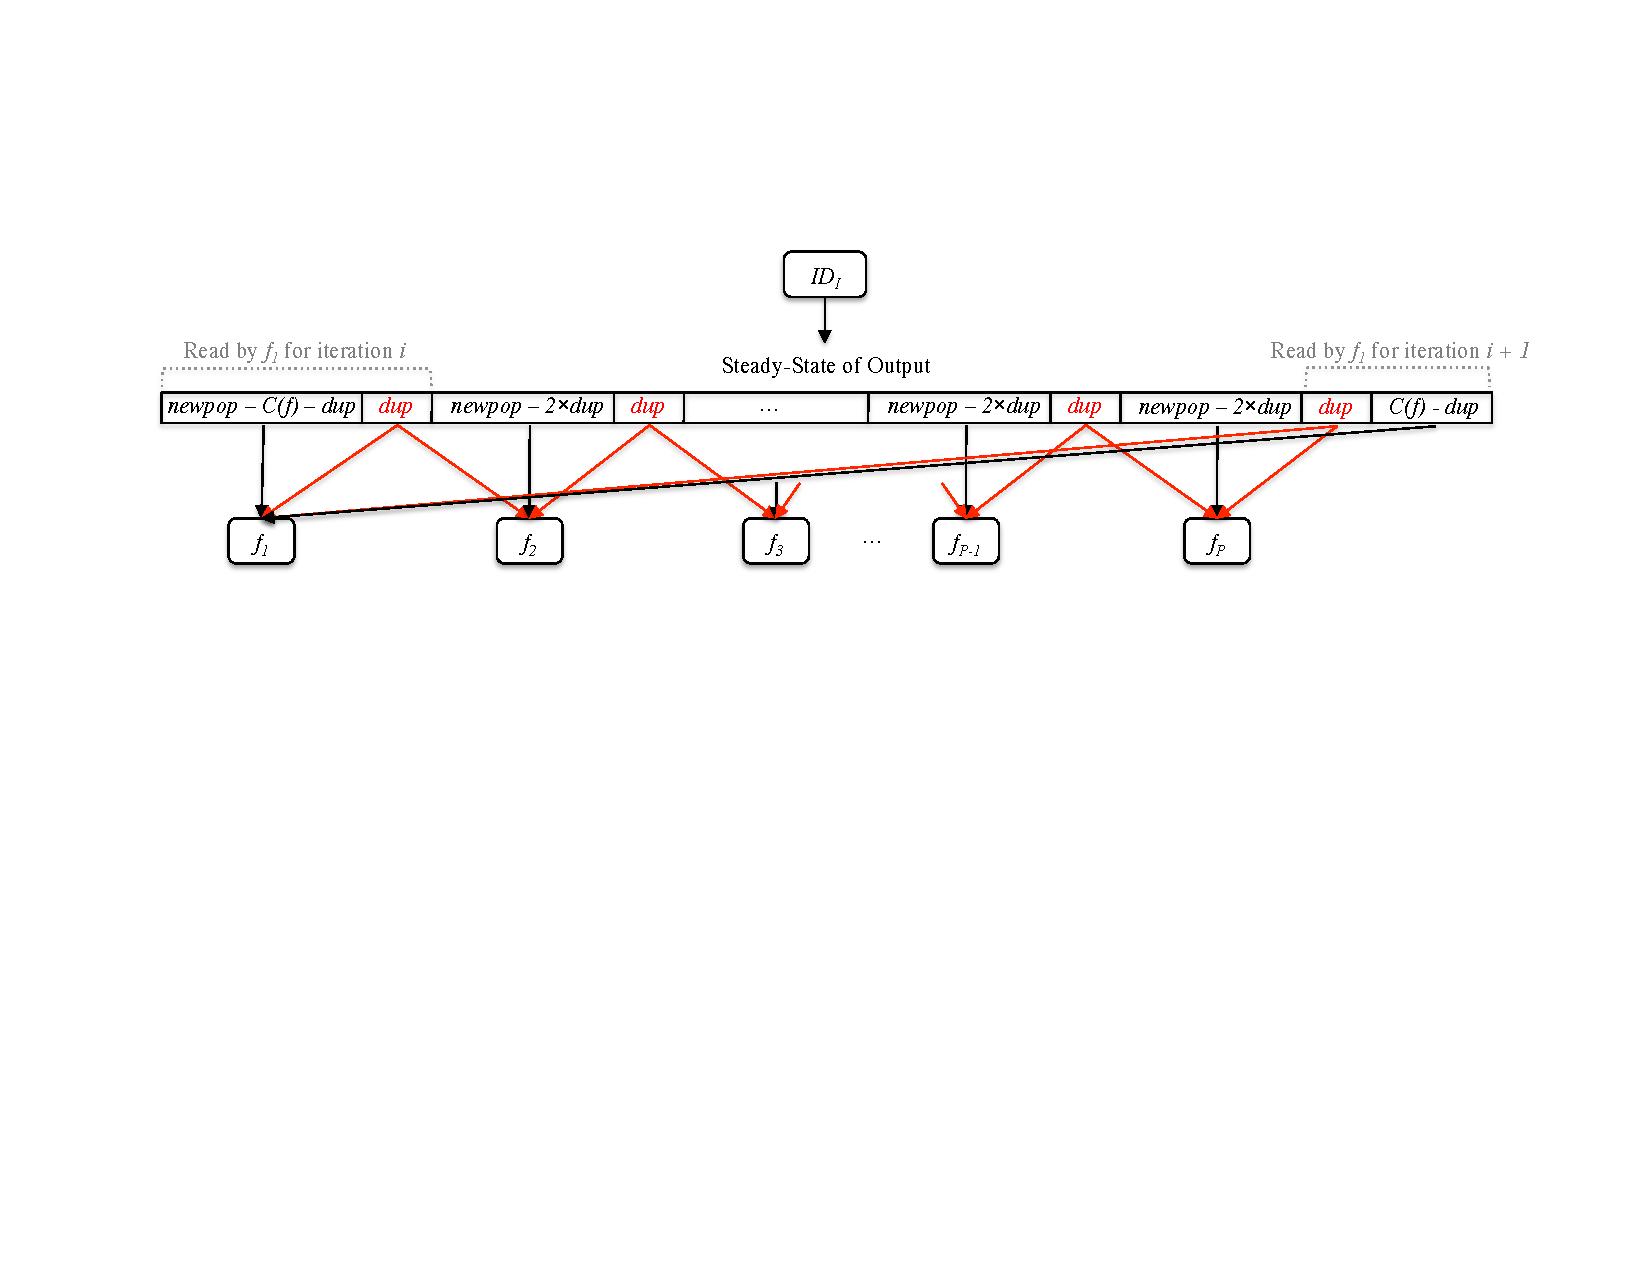
\includegraphics[width=6.3in]{figures/split-pattern.pdf}
\caption[The output distribution required for general
fission.]{
The steady-state output distribution installed for identity node
$ID_I$ by general fission.  Red edges denote items that are shared
across fission products via duplication. If $C(f) > dup$, $C(f) - dup$ items at the end of the
steady-state input are distributed to
$f_1$. \label{fig:split-pattern}}
\vspace{-10pt}
\end{figure*}

The general fission transformation creates two identity nodes ($ID_I$
and $ID_O$) that are encoded to implement the data distribution for
the fission products.  Figure~\ref{fig:split-pattern} illustrates the
pattern of communication between $ID_I$ and the products of $f$.  This
pattern is common to the transformation for all filters we seek to
fiss that meet the preconditions of the transformation.

The fission transformation has the following properties:
\begin{itemize}
\item No item is read by more than 2 fission products.
\item A fission product does not need to remember items across
  steady-state executions of itself. The peeking of the original
  filter $f$ is now encoded in the sharing across fission products
  achieved via the duplication pattern.
\item Only the first fission product $f_1$ is required to receive the $C(f)$
  initialization  items because $C(F) < (M(S,f) / p) \cdot o(W, f)$,
  and it will consume the $C(f)$ items on its first invocation.
\item The presence of the $C(f)$ items in the input buffer after
  initialization must be accounted for by shifting the read pattern
  for the fission products.  The first fission product $f_1$ is offset by
  $C(f)$ items in that it reads its first $C(f)$ items from the
  previous execution stage.  In the steady-state, $f_1$ executing at
  steady-state iteration $i$ shares items with $f_P$ executing at
  steady-state iteration $i-1$.
\item The computation and communication performed by $f$ during the
  initialization stage is transferred completely to the first fission
  product, $f_1$.  
% Since, by construction, only $f_1$ requires the
%   items remaining after the initialization stage.  The other fission
%   products are idle during this stage.
\end{itemize}

% The final steps of the general fission transformation applies
% \textsc{SynchRemove} to remove the identity filters, and stitch the
% communication directly between the fission products and $f$'s
% producer(s) and consumer(s).
 


% To understand the transformation, we first need to understand the item
% distribution and sharing that is required by fission on a filter $f$
% that adheres to the preconditions above.
% Figure~\ref{fig:fission-sharing2} gives another example of the input
% items required by fission products.  In this example, both:

% \[ C(f) = \mt{dup}_f < (M(S,f) / p) \cdot o(W, f) \]
% \[ M(S, f) \mod P = 0\]

% \noindent so $f$ adheres to the preconditions stipulated above for
% general fission.  In the example, the items read for $f$ plus its
% fission products for $P=4$ are shown for the initialization plus two
% steady-states.  After the initialization stage, $C(f) = 2$ items are
% enqueued to the input buffer by the producer(s) to $f$, and $M(S,f)
% \cdot o(W, f) = 16$ items are enqueued by the producer(s) for each
% steady-state.  Examining the sharing requirement for fission products of
% the second steady-state, we can see a pattern emerge with the following
% features:
\section{Analysis}

\begin{figure}[t]
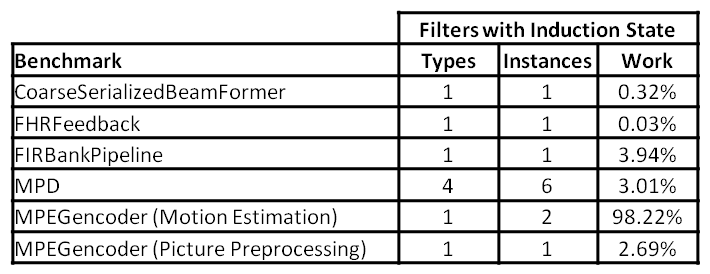
\includegraphics[width=3.5in]{figures/induction-benchmarks.png}
\caption{Benchmarks using induction variable state and estimations on work performed in filters with induction state.\protect\label{fig:benchmarks}}
\end{figure}

Figure~\ref{fig:benchmarks} indicates programs in the StreamIt benchmark suite that use induction variable filters (not including source filters).  The StreamIt compiler provides static estimations of work performed in filters.  The above table indicates the work performed in specifically the induction variable filters.

The majority of programs do not have substantial work performed in filters using induction variables, the MPEG-2 motion estimation subset being the exception.  However, eliminating state will have a large impact on runtime performance even on programs with low work concentration in stateful filters.  We model the potential speedups of a particular stateful program in this section.  For the purpose of this analysis, we will assume no communication cost between filters.  We will also assume the compiler exposes no pipeline parallelism.  This assumption forces the serialization of stateful filters on the stream graph.

Let $N$ be the number of cores we are planning to parallelize over.  Let $\sigma$ be the percentage of work performed in stateful filters that can have its state eliminated, in this case solely filters that use induction variable state.  

If $\sigma = 0$, the entire program is stateless.  The program can be fused to coarsen the granularity, then fissed and mapped to all of the available cores.  Each core would perform $\frac{1}{N}$ of the total work.  Thus with no state, the program can exhibit speedups of up to $N$ times the single-core runtime.

For filters that contain stateful work, we describe the program in terms of work that can be parallelized with work that cannot be parallelized.  $1-\sigma$ of the work in the program is considered stateless, and thus can be fissed and assigned to $N$ individual cores.  The stateful filters cannot be parallelized, and is sequential to all work in the program.  The total serialized work is $\frac{1-\sigma}{N} + \sigma$.  Thus the total speedup is the amount of work done without parallelization, or 100\% of the work, divided by the new parallelized work.  
\begin{eqnarray*}
\dfrac{1}{\frac{1-\sigma}{N} + \sigma} &=& \dfrac{N}{1 + \sigma(N-1)}
\end{eqnarray*}

We can characterize the amount of speedup between a completely stateless program to an equivalent stateful program with $\sigma$ percentage of stateful work.  This is simply:
\begin{eqnarray*}
\dfrac{N}{\frac{N}{1 + \sigma(N-1)}} &=& 1 + \sigma(N-1)
\end{eqnarray*}



\begin{figure}[t]
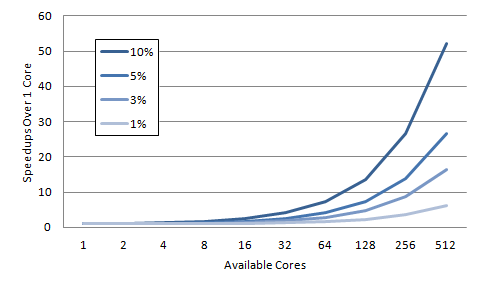
\includegraphics[width=3.5in]{figures/theoretical-speedups.png}
\caption{Theoretical speedups for stateless filters over corresponding stateful filters with $\sigma$\% work.  \protect\label{fig:theo-speedups}}
\end{figure}

Figure~\ref{fig:theo-speedups} indicates the potential speedups over stateful programs given stateful work percentages and a varying number of cores.  Even benchmarks in the suite that exhibit only 3\% work in stateful filters can exhibit 8x speedups with 256 cores.  Providing a means to remove state from filters that exhibit very small amounts of work relative to the rest of the program can still generate substantial speedups in the near future.



\begin{figure}[t]
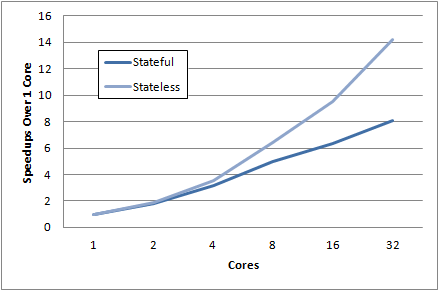
\includegraphics[width=3.5in]{figures/firbank-results.png}
\caption{Speedups for FIRBankPipeline, with and without induction variable state.  \protect\label{fig:firbank-results}}
\end{figure}

FIRBankPipeline contains one filter that uses induction variable state.  According to Figure~\ref{fig:benchmarks}, there is 3.94\% of work performed in the induction filter, which represents the only state in this benchmark.  Figure~\ref{fig:firbank-results} indicates the speedups over 1 core for both stateful and stateless implementations.  Between stateful and stateless implementations, there is 1.35X speedup on 8 cores, 1.58X speedup on 16 cores, and 1.84X speedup on 32 cores, which abides fairly closely to the model.
\section{MPEG-2 Motion Estimation Subset}


\begin{figure}[t]
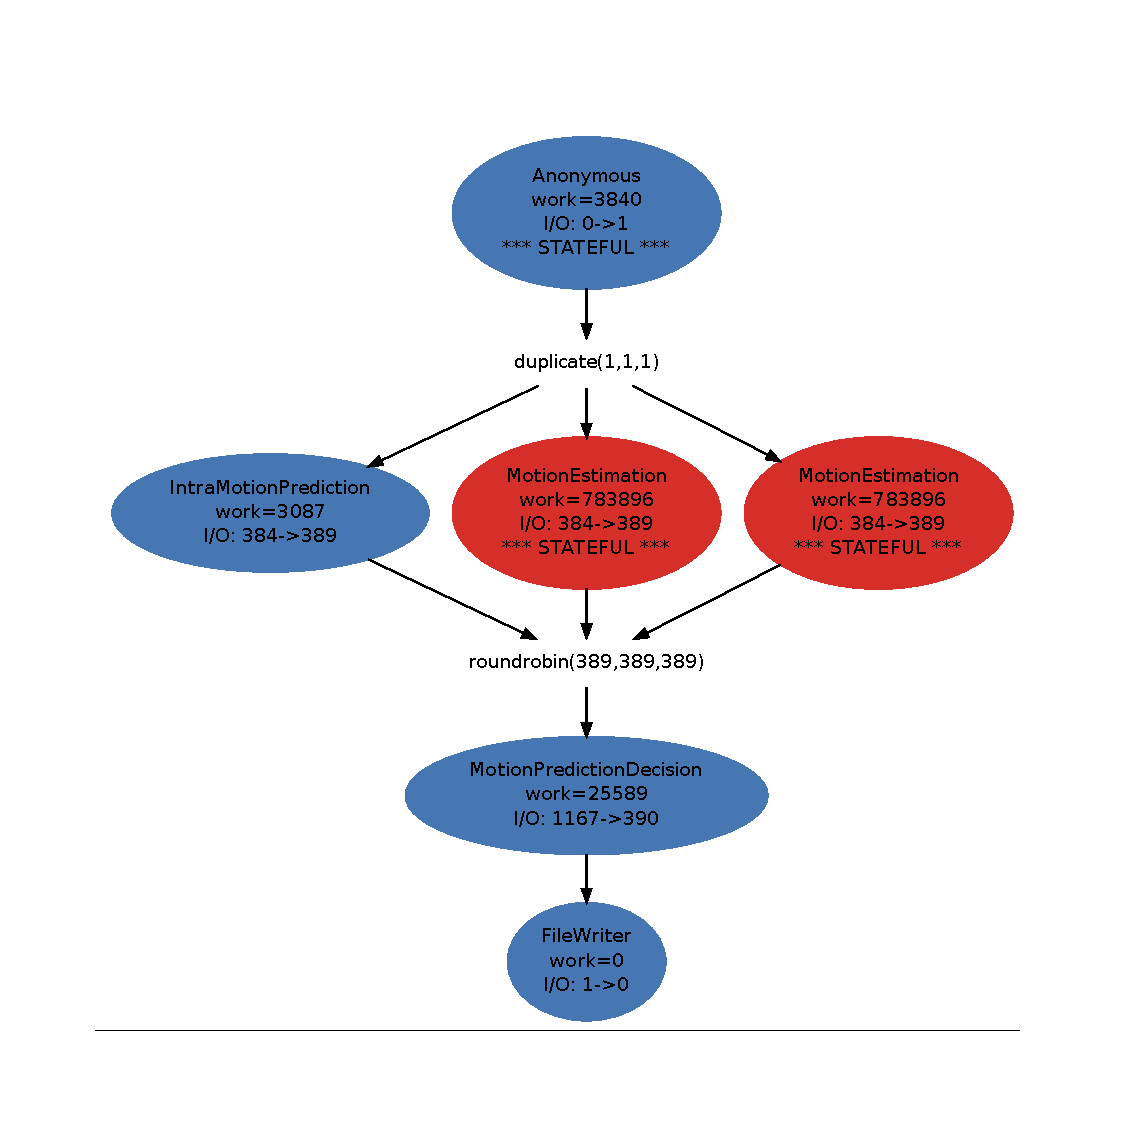
\includegraphics[width=3.5in]{work_estimate_mpeg_motionestimation.pdf}
\caption{MPEG Motion Estimation stream graph.\protect\label{fig:mpegMEgraph}}
\end{figure}


This section presents an application of induction variables to the Motion Estimation compression subset of the MPEG-2 encoder.  MPEG-2 is a standard for coding moving pictures and audio information and has a wide variety of multimedia applications.  

The specification contains various types of compression, one of which is motion prediction.  Motion prediction is a lossless compression, or one that eliminates redundant information from a signal while allowing for an exact reconstruction.  Motion prediction takes advantage of the fact that frames of a video contain a large amount of temporal redundancy.  A particular video sequence often contains duplicated scenes between consecutive frames.  Motion estimation attempts to generate motion predictions with respect to a set of reference frames.  These reference frames can be obtained from previous pictures or from both previous and future pictures.  Accordingly, the MPEG-2 encoder can utilize forward and backward motion estimation to achieve this form of compression.

The MPEG-2 standard organizes pictures into 16x16 groups of pixels called macroblocks.  Each macroblock is itself comprised of four 8x8 blocks of pixels termed as blocks.  Macroblocks can be encoded without any motion prediction, known as intra coded pictures, with only forward motion prediction, known as predictive coded pictures, and with both forward and backward motion prediction, known as bidirectionally predictive coded pictures.  These macroblocks are the basis of MPEG-2 motion prediction.  

The process of Motion Estimation entails comparing macroblocks between frames.  The motion estimator forms a motion vector that indicates a cartesian displacement of the macroblock from the most similar macroblock in the reference frames.  The matching macroblock is also removed from the new macroblock, yielding a residual macroblock that contains the difference between the prediction and the actual macroblock being encoded.  

The Motion estimation stream subgraph of the MPEG-2 encoder is illustrated in Figure~ref{mpegMEgraph}.  Each macroblock will be tested against all three types of prediction (intra coded, forward predicted, and backward predicted) to determine which is the best method for motion estimation.  The MotionEstimationDecision filter determines of these results, which is the best encoding technique.

[cite madrake meng 06]

The work estimation of this compression indicates the filter MotionEstimation is stateful and contains the majority of the work.  The duplicate splitjoin sends a copy of the picture to both forward and backward MotionEstimation and IntraMotionPrediction.  

The MotionEstimation filter pulls macroblocks at a time, iterating through a two-dimensional array (16x16 macroblocks) along the picture.  The filter relies on induction variables to maintain its array position.  We can apply the induction variable transformation on this filter to remove the state in the filter.

Reference pictures are set using upstream messaging from later in the stream graph.  Currently the backend does not support the use of upstream messaging, so for the purpose of benchmarking this application, the reference picture is set to a dummy value and is unchanged throughout the program.  This does not detract from the data parallelism introduced after removing the induction state.  Upstream messaging would simply require that sent messages be duplicated to all fissed filters in the stream graph.

Figure~ref{} shows the runtime figures for the original stateful MPEG-2 motion estimation subset compared to the stateless subset.  We can see significant improvements to runtime after making this subset stateless.  
%\section{Implementation}

Filters that use induction variables inherently use state to keep track of
how often it has been called through the span of the program.  We attempt 
to remove this user-facing state by introducing an iteration keyword to the 
StreamIt language.  Functionally, this iteration keyword returns how often 
the work function of the corresponding filter has been called.  Filters 
using this feature are no longer classified as stateful in the StreamIt
compiler, as the compiler has the means of fissing these filters in a 
predictable manner.

In translating higher level code into the intermediate representation, the 
iteration keyword is desugared.  The compiler adds an internal induction 
variable field for filters that use the iteration keyword.  This induction
variable is incremented at the end of each \texttt{work} call.  Any instance
of the iteration keyword is translated into a reference to this internal 
induction field.  

This desugaring process introduces induction variable state to the intermediate
representation of the filters.  Modifications must also be made to the fission 
process to allow the compiler to fiss these stateful filters and ensure 
consistency between fission products after fission.  

The fission process now modifies the fission products by adding the 
following values as fields of the products:
\begin{itemize}
	\item \texttt{start}: the value of the induction variable each product starts with.
	\item \texttt{reps}: how often the \texttt{work} function of the product is 
	  called between rounds.
	\item \texttt{total}: the sum of all reps of all fission products. This value is 
	  the same amongst all fissed products.
\end{itemize}
Accordingly, each fission product should start each round with induction values
of
\begin{center}
\texttt{total}*\texttt{n} + \texttt{start}
\end{center}
and range up to the value
\begin{center}
\texttt{total}*\texttt{n} + \texttt{start} + \texttt{reps} - 1
\end{center}
where \texttt{n} is a nonnegative integer indicating how many rounds have
been run in the span of the program.  We have to account for the off-by-one
error as the first iteration is run.

At the end of each fission product \texttt{work}, after incrementing the 
induction value, a check must be made to see if it is necessary to increment 
the induction variable to the next round of  values.  This will prevent certain
fissed products from making calls with duplicate induction values.  
\begin{center}
\texttt{iter} - \texttt{start} - \texttt{reps} \% \texttt{total} == 0
\end{center}
The fissed products must check that the current induction value less the 
\texttt{start} and \texttt{reps} of that fissed product is divisible by the 
\texttt{total}.  This is consistent with the maximum value per round as 
indicated above.  Once the fissed product's induction value has reached 
this value, it must be set to:
\begin{eqnarray*}
\texttt{iter}_{n+1} &=& \texttt{iter}_{n} + (\texttt{total} - \texttt{reps}) \\
&=& (\texttt{total}*\texttt{n} + \texttt{start} + \texttt{reps}) \\
&&  \ \ +\ (\texttt{total} - \texttt{reps}) \\
&=& (\texttt{total}*(\texttt{n+1}) + \texttt{start})
\end{eqnarray*}
which is the starting iteration value of the next round, as defined.

The scheduler may also modify the multiplicity of the rounds.  The field values
added to the fissed products must, in turn, be updated to reflect this change.
Since all fissed products will be multiplied by the same steady multiplicity
factor, we can simply multiply each of the \texttt{start}, \texttt{reps}, and 
\texttt{total} values by the same steady multiplicity value.



%\section{Model of Computation}
\label{model}

The model of computation employed for this paper is a general model
that is agnostic of input language.  The semantics of the model are
built upon synchronous dataflow (SDF)~\cite{leeSDF}.  Although
inspired by the StreamIt programming language, the model can represent
aspects of other streaming languages such as Brook~\cite{brook04},
Lime~\cite{lime10}, SPL~\cite{spl09} and SPUR~\cite{spur05samos}.
Consider a directed graph $G = (V, E)$ corresponding to a streaming
application. $F \in V$ is a filter in the application and $(f, g) \in
E$ is an edge (or {\it channel}) in the graph that denotes
communication from $f$ to $g$ using a FIFO channel.  Each filter is
described by rate declarations, data reorganization patterns,
and compute functions as described below. The techniques in this paper
require static-rate graphs, i.e., all of the quantities of the filters
are statically determinable.

%  Figure~\ref{fig:streamgraph} gives an example
% stream graph for a FM radio with an equalizer.  The figure also
% includes details for two of the filters; the details are explained
% below.

% The filter is the basic unit of execution in our model.  Each filter
% is described by multiple rate declarations, data reorganization
% patterns, and compute functions.  Basically, each filter defines the
% number of items it consumers and produces each time it is executed.
% The execution of a stream graph is represented by a {\it schedule} of
% a graph $G$.  A schedule gives a multiplicity for each filter $F \in
% V$ that denotes how many times to fire filter $F$.  When a schedule is
% executed, each filter fires when it has buffered enough input to
% satisfy its input requirement (a filter will not fire more times than
% given by a schedule).  In our notation, a schedule is represented by
% the variable $\Sigma$, and it denotes a mapping from filters to
% non-negative integers. The multiplicity of filter $F$ in schedule
% $\Sigma$ is denoted by $M(\Sigma, F)$.

For each filter, $F \in V$, a {\it work} function, $W_F$, is defined.
The work function defines the atomic execution step for each filter.
For each filter, $F \in V$, a {\it prework} function, $W_F^P$, can
also be defined.  Prework describes a computation step that executes
once at the first firing of a filter.  The prework function is
executed only once per execution of the {\it application}; it
describes any special initialization behavior required for a
filter. We denote a function with the variable $\mathcal{F} \in \{W^p,
W\}$.  We sometimes leave out the subscript that denotes the filter if
it is clear which work or prework function is intended.

For each filter $F \in V$ we define the following:
\begin{itemize}

\item $o(\mathcal{F}, F)$, or {\it pop} rate, is the number of items
  dequeued from $F$'s input buffer per firing of $\mathcal{F}$.

\item $e(\mathcal{F}, F)$, or  {\it peek} rate, 1 $+$ the greatest index that is read (but
  not necessarily dequeued) from $F$'s input buffer per firing of
  $\mathcal{F}$. 

\item $u(\mathcal{F}, F)$, or {\it push} rate , the number of items enqueued to $F$'s
output buffer per firing of $\mathcal{F}$.  

\end{itemize}

\noindent Sliding window filters have a peek rate greater than the pop
rate.  We somethings refer to sliding window filters as {\it peeking}
filters. Figure~\ref{fig:pipeline-example}(a)
demonstrates a peeking filter.  The figures shows that the window of
items read for 3 consecutive firings of the filter overlap.  For the
work function execution, a peeking filter $F$ requires $e(W_F, F)$
items to be on its input channel(s) to fire.  $F$ will consume
(dequeue) the first $o(W_F, F)$ items after the firing of the work function.

\begin{figure}[t]
\centering
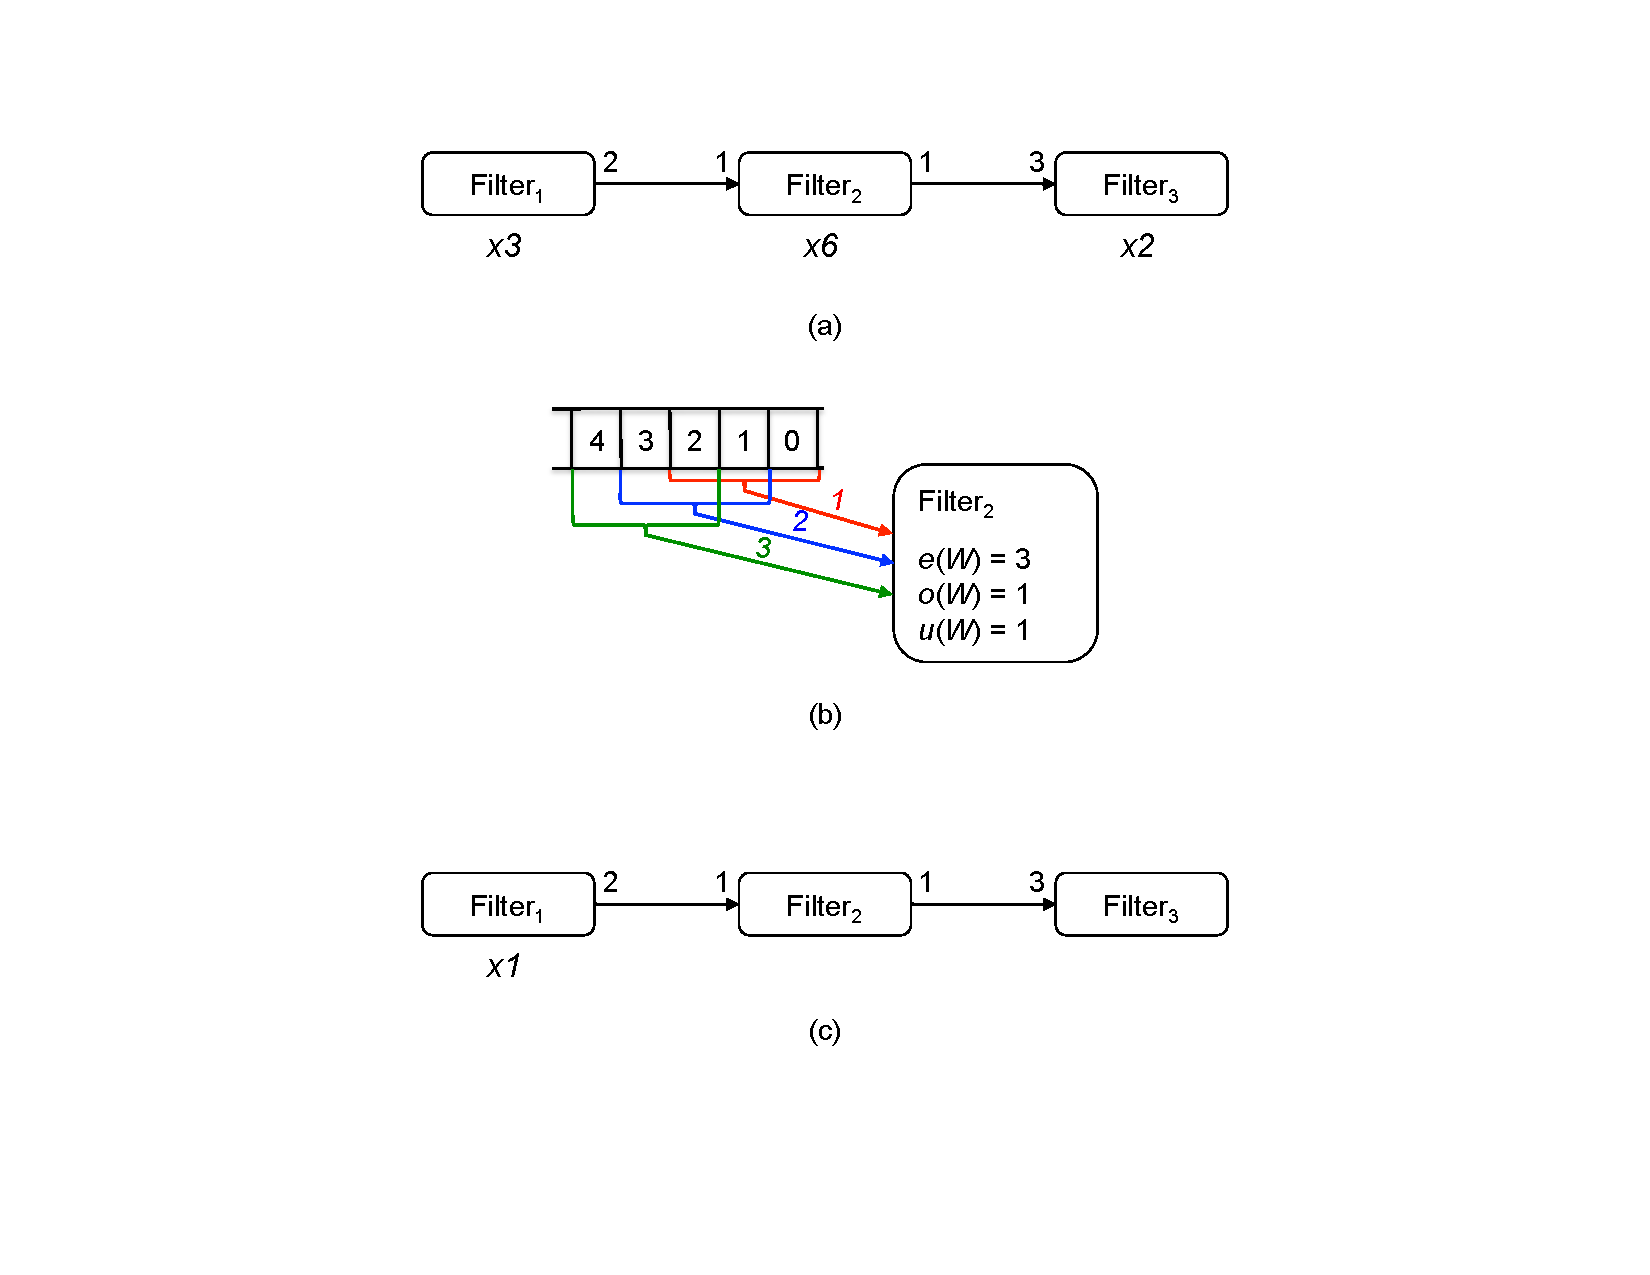
\includegraphics[width=3.0in]{figures/pipeline-example.pdf}
\caption[A pipeline of three filters with schedules.]{ (a) gives
  details for a sliding window filter.  The figure
  shows the window of items read for 3 consecutive firings of the
  filter.  Notice the overlapping in the windows.  (b) presents a pipeline of
  three filters with push and pop rates.  (b) also gives a
  legal steady-state schedule and initialization schedule for the
  three filters. $C(\mt{Filter}_2) = 2$ and
$C(\mt{Filter}_1) = C(\mt{Filter}_3) = 0$. 
  \label{fig:pipeline-example}}
\vspace{-10pt}
\end{figure}

A schedule gives a multiplicity for each filter $F \in V$ that denotes
how many times to fire filter $F$. A {\it steady-state schedule} can
be calculated such that all filters fire in the schedule, and the
schedule can be repeated indefinitely~\cite{lee87}.  Steady-state
execution of the graph entails repeating the steady-state schedule for
as much input as is expected.  Execution of the stream graph is
conceptually wrapped in an outer loop that continuously executes the
steady-state schedule.  Figure~\ref{fig:pipeline-example}(b) gives an
example of a steady-state schedule calculated for a graph that
consists of three filters in a pipeline.  All the multiplicities of
the steady-state can be multiplied by the same constant $c$, and the
result will still be a valid steady-state.  We call this process {\it
  increasing} the steady-state of the graph by $c$.

Our model does not deal with arbitrary schedules of filter executions.
The steady-state schedule, $S$, is explicitly represented.
Furthermore, an {\it initialization} schedule, $I$, is explicitly
represented that enables the steady-state schedule in the presence of
peeking filters.  An initialization schedule is required if peeking is
present in a graph to enable the calculation and execution of a
steady-state schedule~\cite{karczmarek-lctes03}.  After the initialization
schedule executes, each filter $F$ is guaranteed to have at least
$e(W_F, F) - o(W_F, F)$ items in its input buffer.
Figure~\ref{fig:pipeline-example}(b) gives a legal initialization
schedule for the pipeline that enables the peeking in filter
$\mt{Filter}_2$.  During application execution, the initialization
schedule is executed once followed by an infinite repetition of the
steady-state schedule.  The number of items remaining on $F$'s input
channel(s) after execution of the initialization schedule is
represented by $C(F)$.

In our notation, a schedule is represented by the variable $\Sigma$,
and it denotes a mapping from filters to non-negative integers. In our
execution model, only an initialization schedule and a steady-state
schedule are considered (thus $\Sigma \in I,S$). The
multiplicity of filter $F$ in schedule $\Sigma$ is denoted by
$M(\Sigma, F)$.  

A filter may have multiple incoming edges and/or multiple outgoing
edges.  Filter inputs are organized into a single internal FIFO buffer for the
filter to read according to an {\it input distribution pattern}, and
filter outputs are distributed from a single internal output FIFO
buffer according to an {\it output distribution pattern}.   
The input distribution pattern is represented as:
{\ninepoint
\[ \mt{ID}(\Sigma, F) \in (\mathbb{N} \times E)^n = ((w_1,e_1), (w_2,
e_2), ..., (w_n, e_n))\]
}
\noindent Where $n$ is the width of the input distribution pattern.
The input distribution describes the round robin joining pattern for
organizing the input data into the filter's single internal FIFO
buffer, where $w_i$ items are received from edge $e_i$ before
proceeded to the next edge, $e_{i+i}$.

The output distribution pattern describes both round-robin
splitting and duplication in a single structure:
{\ninepoint
\[ \mt{OD}(\Sigma, F) \in (\mathbb{N} \times (P(E)-\emptyset))^m = ((w_1,d_1), (w_2,
d_2), ..., (w_n, d_n))\]
}
\noindent Where $P(E)$ is the powerset of $E$.  Each $d_i$ is called
the {\it dupset} of weight $i$.  The dupset $d_i$ specifies that $w_i$
items be duplicated to the edges of the dupset.  Each tuple denotes
that $w_i$ output items of $F$ are duplicated to the edges of $d_i$
before moving on to the next tuple.

\begin{figure}[t]
\centering
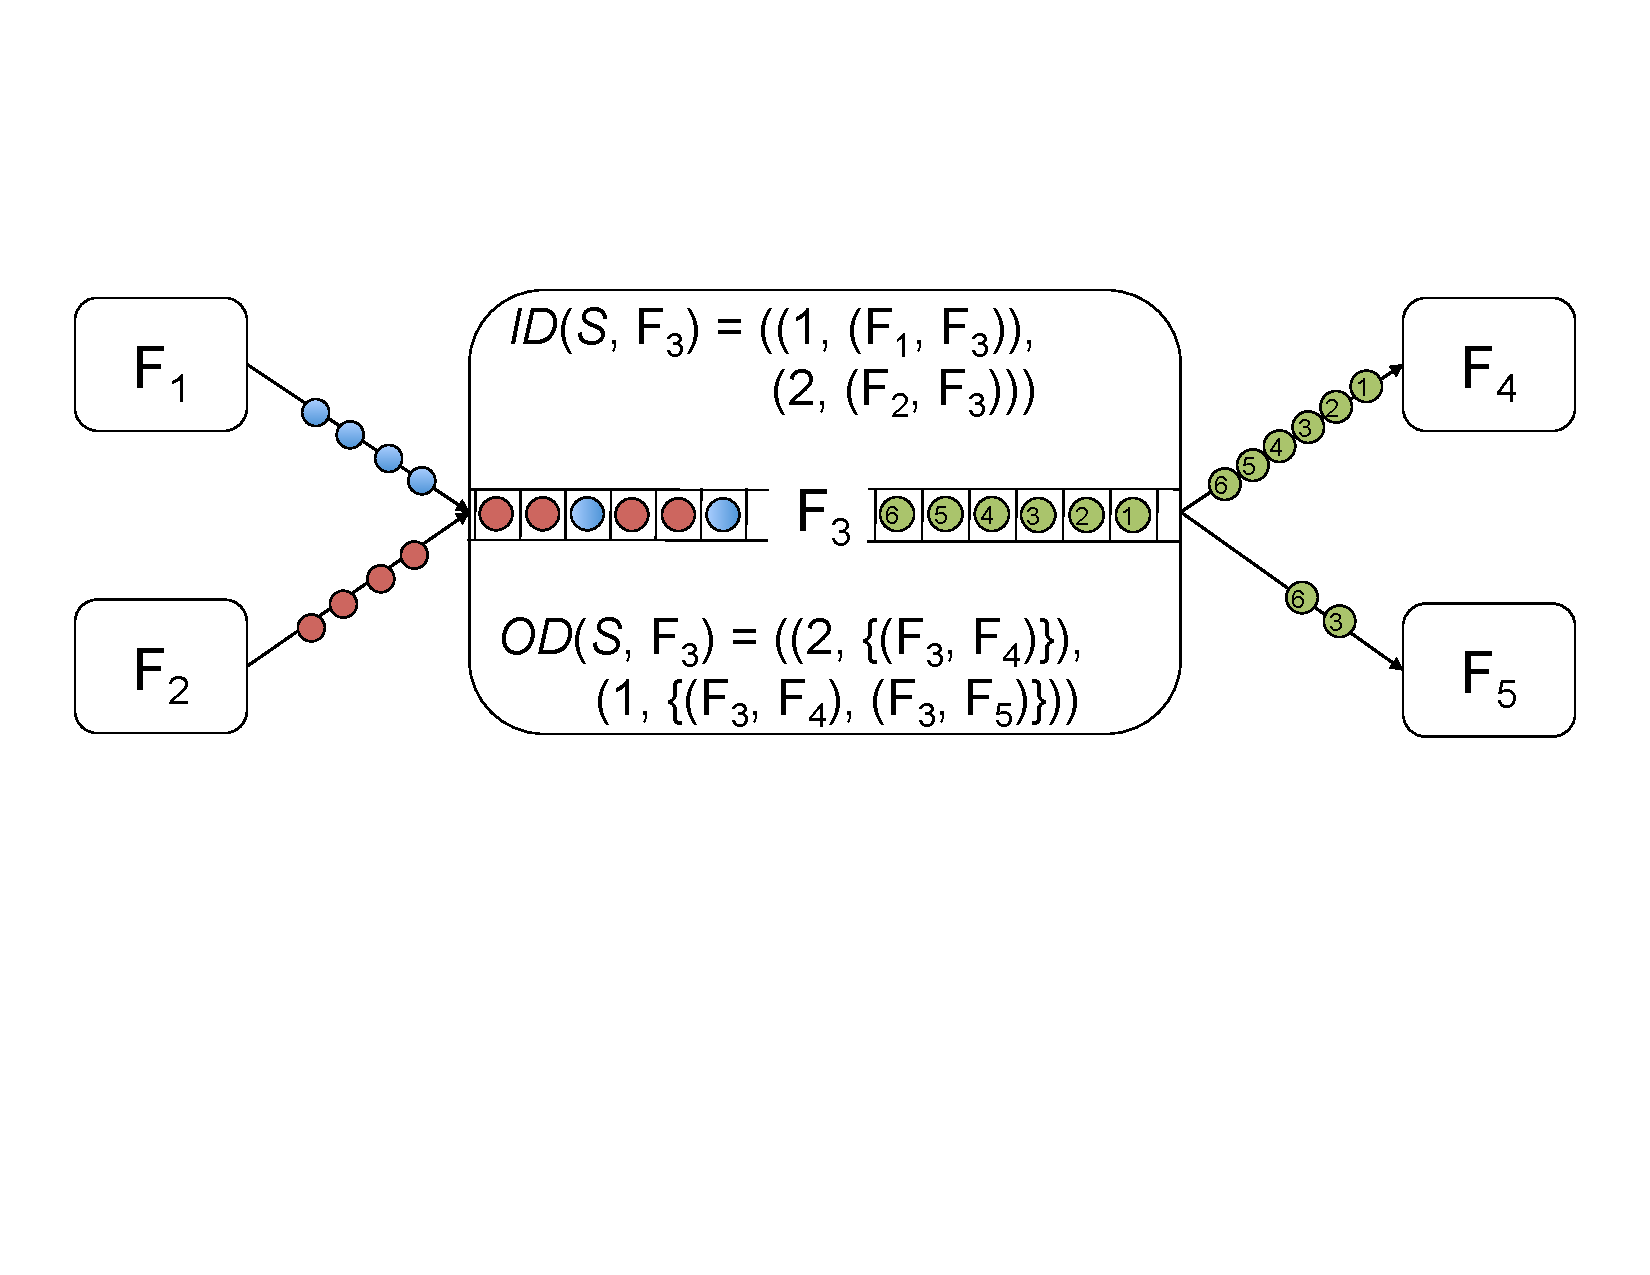
\includegraphics[width=3in]{figures/dist-example.pdf}
\caption[Example of input and output distribution.]{
An example of a filter with non-trivial input and output distribution patterns.
Filter $F_3$ has both multiple inputs and multiple outputs.  The input
items from the multiple inputs are joined in the pattern described by
its input distribution ($ID$): receive 1 item from $F_1$ and 2
items from $F_2$, and repeat.  $F_3$'s output items are distributed to
its multiple outputs as described by the output distribution pattern
($OD$):  2 items to $F_4$, then 1 item is duplicated to both $F_4$ and
$F_5$.  The output items of $F_3$ are indexed to show how they are
distributed to $F_4$ and $F_5$.
\label{fig:dist-example}}
\vspace{-10pt}
\end{figure}

The input and output distributions are repeated as needed for the
schedule that is being executed.  The start of each steady-state
iteration resets the input and output distributions to the first tuple.
Figure~\ref{fig:dist-example} highlights an example of a filter with
both multiple inputs and multiple outputs, and how the distribution
patterns translate into scattering and gathering.

Let $\mt{RO}(F_1, F_2, \Sigma)$ be the ratio of output items $F_1$
splits along the edge $(F_1, F_2)$ to the total number of items that
$F_1$ produces in the schedule $\Sigma$.  This can be calculated from
$F_1$'s output distribution pattern for $\Sigma$.  For example, in
Figure~\ref{fig:dist-example}, $\mt{RO}(F_3, F_4) = 1$ and
$\mt{RO}(F_3, F_5) = \frac{1}{3}$.  Conversely, let $\mt{RI}(F_1, F_2,
\Sigma)$ be the percentage of total input items that $F_2$ receives
from $F_1$ for $\Sigma$.  For example, in
Figure~\ref{fig:dist-example}, $\mt{RI}(F_2,F_3) = \frac{2}{3}$.

% Let $s(\mathcal{F}, F)$ denote the execution time (in cycles, with
% respect to a given real or conceptual machine) of function
% $\mathcal{F}$ of filter $F$.  For many of the static scheduling
% techniques covered in this thesis, we calculate a static estimation of
% the total amount of work for a filter $F$ in the steady-state, $s(W,
% F) \cdot M(S, F)$.  We often use the term {\it work estimation} to
% denote this quantity.

%\section{Sliding Windows and Data Parallelization}

\begin{figure*}[t]
\centering
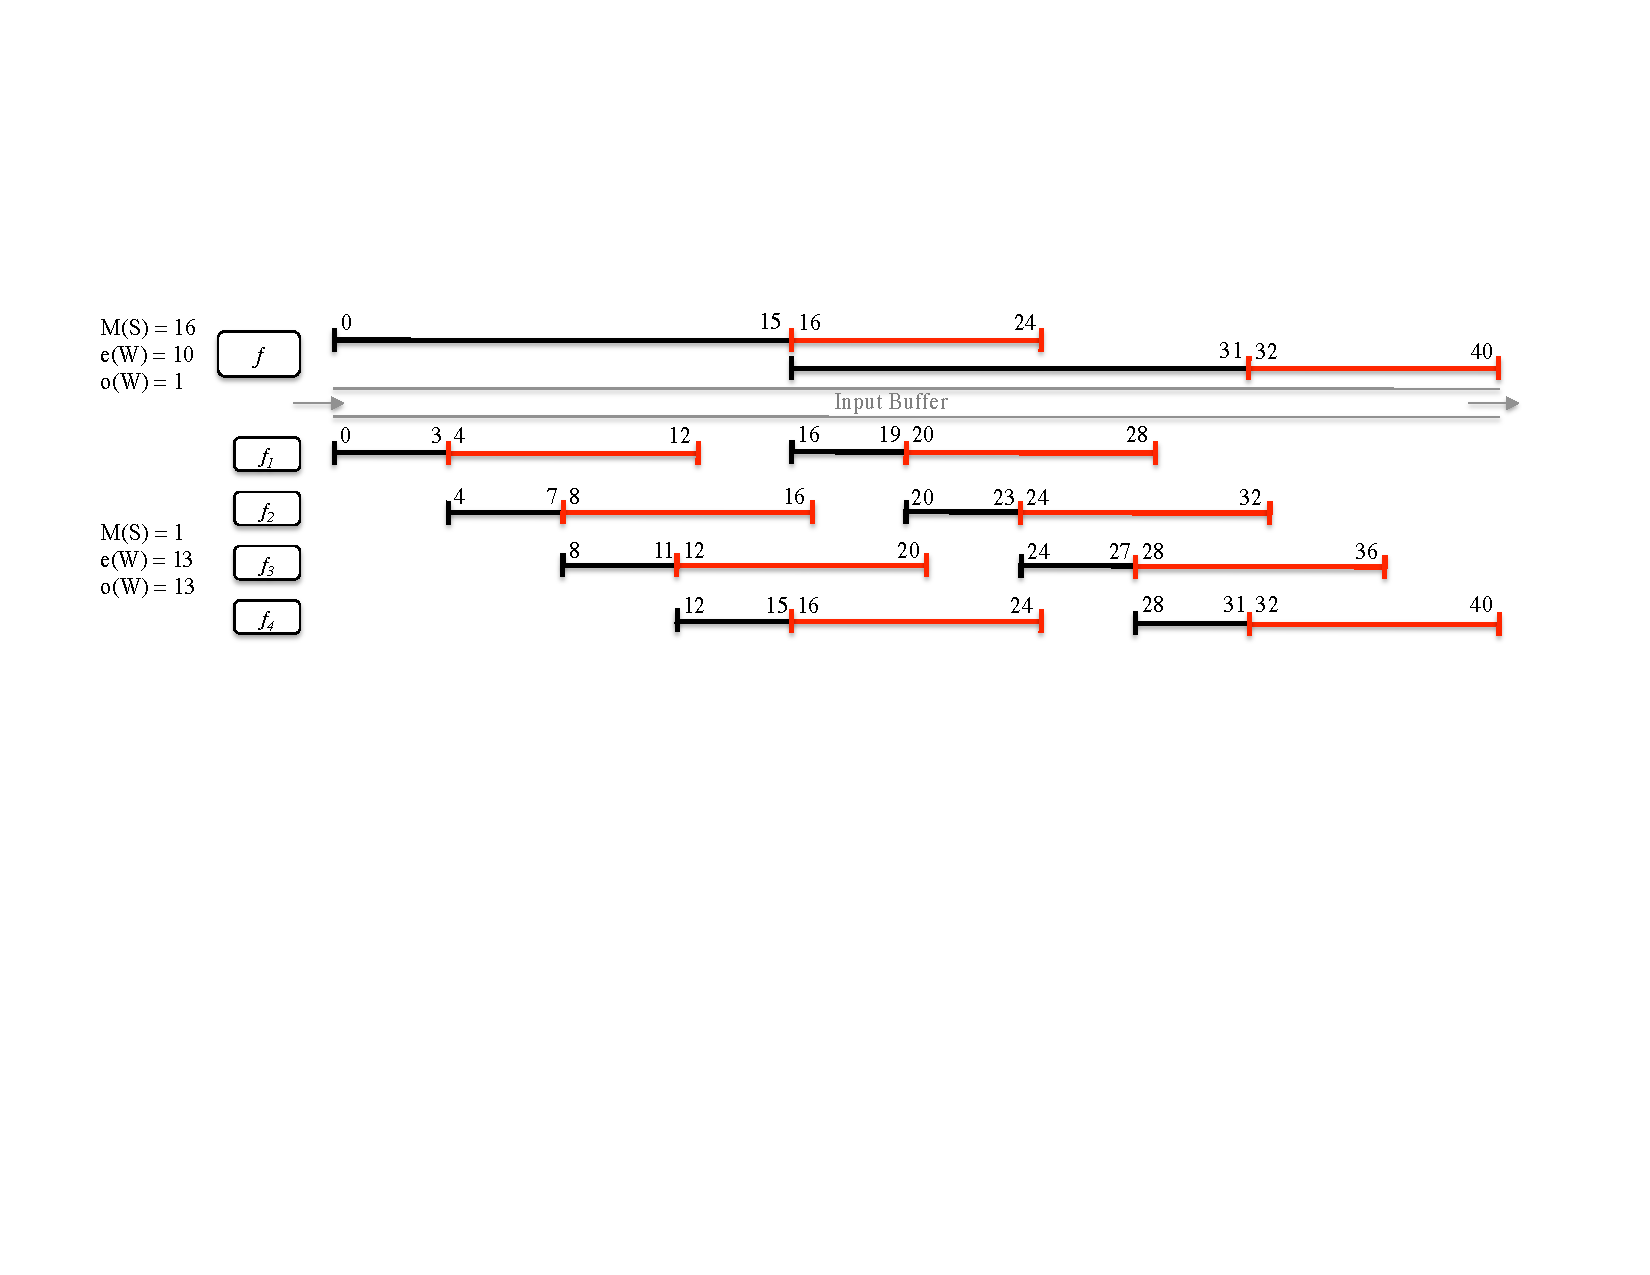
\includegraphics[width=6.0in]{figures/fission-sharing.pdf}
\caption[An example of the sharing required by fission.]  { An
  example of the duplication of items required by fission.  Filter $f$
  is fissed by 4 into $f_1$ - $f_4$.  Two steady-states of the item
  indices required for both $f$ and the fission products are shown.
  Item indices that are inspected but not dequeued are in red.  For the
  fission products, it is required to duplicate 1 out of 4 items to
  all 4 filters, and the remaining 3 items are duplicated to 3
  filters.  Notice that the number of items inspected by the fission
  products is the same as $f$, but the total number of items dequeued 
per steady-state is split across the $f_i$s.
\label{fig:fission-sharing}}
\end{figure*}


For sliding window filters, some (or all) input items are required by
multiple iterations.  Without explicit support for sliding window
computations, shared items must be manually saved for a later
iteration.  Figure~\ref{fig:fir-nopeeking} demonstrates a manual
implementation of a sliding window.  This implementation is very
difficult for a compiler to analyze and parallelize.  Obscuring the
data parallelism in sliding window computations limits parallelization
scalability.  For our benchmarks, ChannelVocoder, Filterbank, and
FMRadio, stateful implementations of sliding window filters limits
theoretical parallelization scalability to 18, 37, and 14 cores, respectively.
Figure~\ref{fig:fir-peeking} gives an implementation of an FIR filter
that utilizes StreamIt's peeking idiom.  The behavior of the sliding
window is described by the pop and peek rates.  The window is accessed
via the {\tt peek(i)} expression.  Exposing sliding windows in this
manner enables the techniques presented in this paper thus enabling
scalable parallelization to at least 64-cores.

\begin{figure*}
\centering
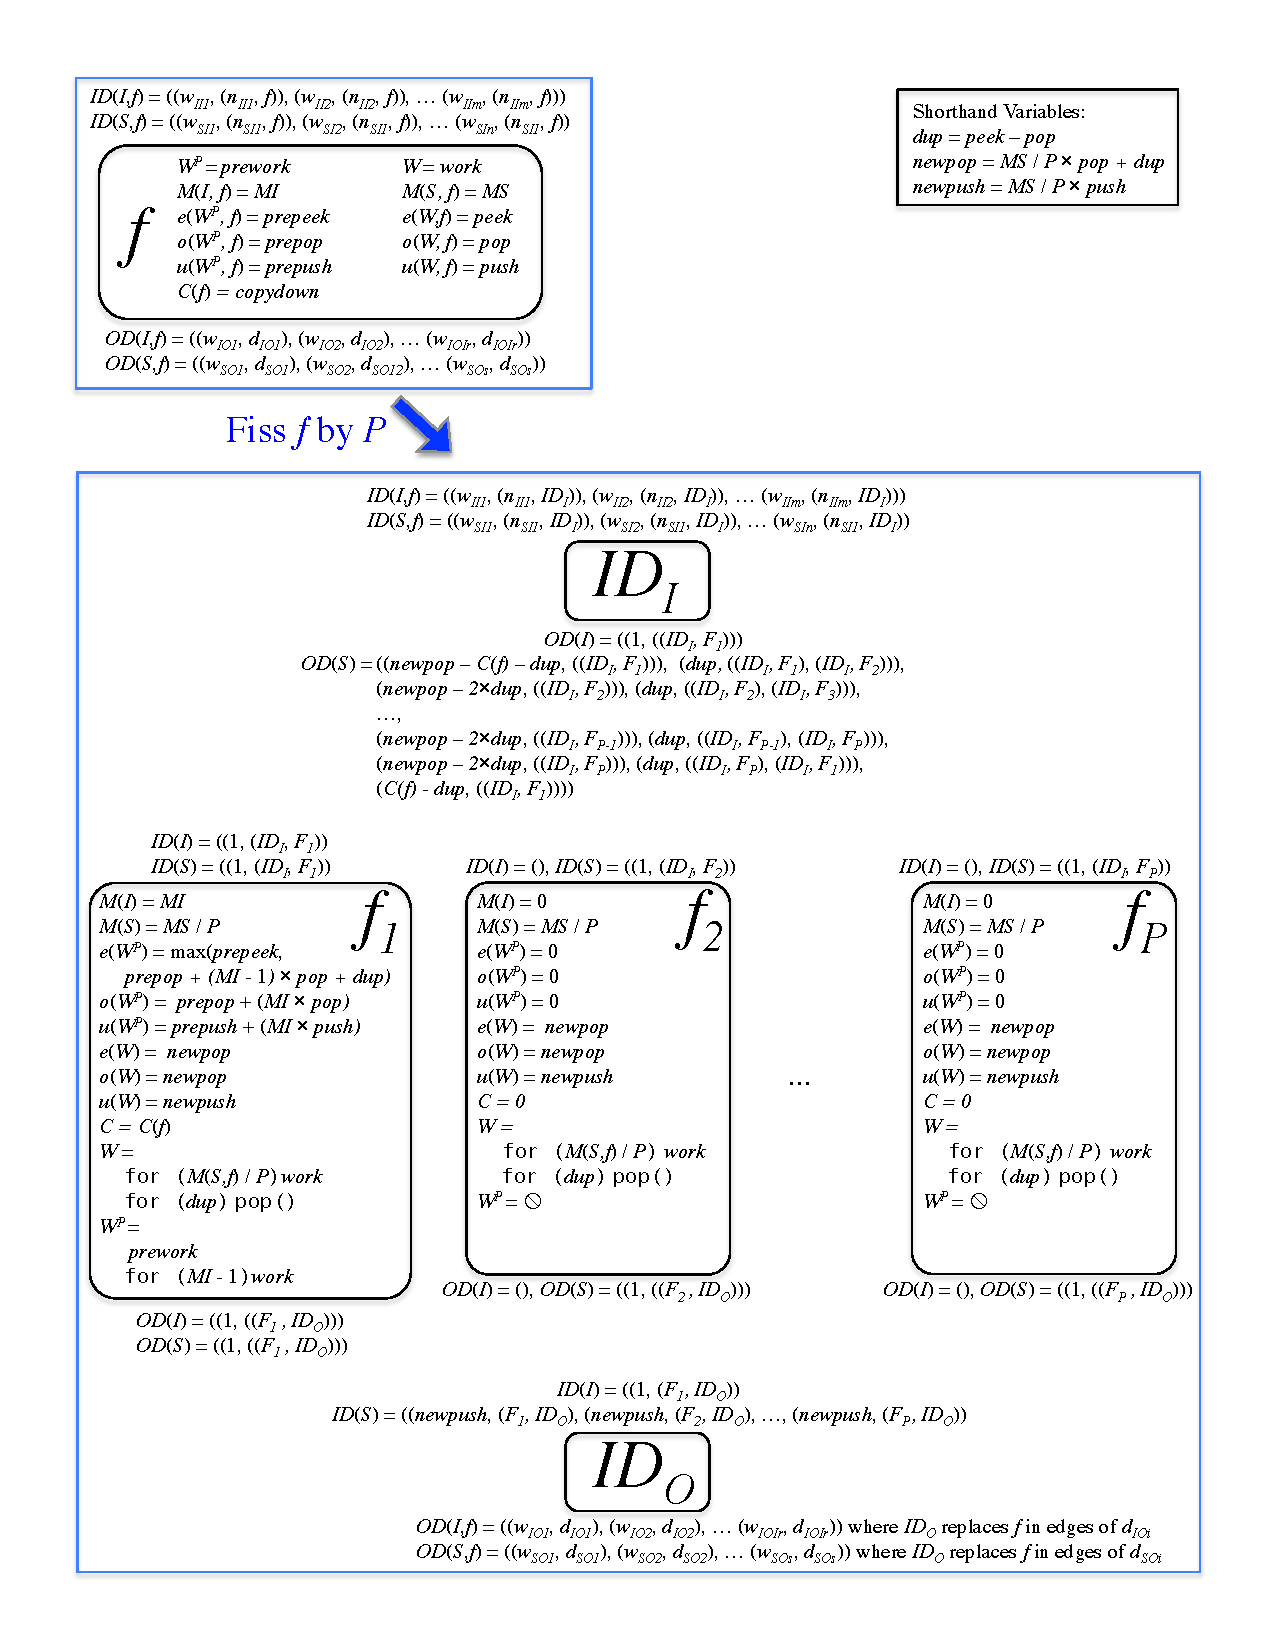
\includegraphics[width=\textwidth]{figures/general-fission.pdf}
\caption[Fission of a node in the general stream graph.]{Fission of a
  node $f$ by $P$ in the general stream
  graph.\label{fig:general-fission}}
\end{figure*}


Data parallelization is possible if the compiler can reason about the
sharing requirement of the sliding window filter.  When a sliding
window filter is parallelized via the process of fission, the window
state inherent between iterations is transformed into the
communication of shared items to multiple products of the filter.
Figure~\ref{fig:fission-sharing} gives an example of the sharing
requirement between fission products for a fission application. 
Previous work implements fission of sliding window filters via
duplication of all input items to all fission products and decimation
of unneeded items at each product filter~\cite{streamit-asplos}.  We
call this technique {\it DupDec}. If each product is mapped to a
distinct core, the replication of items requires inter-core communication.

The efficiency of DupDec depends on the application being mapped and
the communication mechanism of the target.  Two of our benchmarks
include significant amounts of {\it unnecessary} duplication in the
steady-state when DupDec is utilized by the techniques described
in~\cite{gordon-asplos06}:

\begin{itemize}
\item ChannelVocoder: 5,200 of 13,336 total items (38\%)
\item FMRadio: 1,108 of 1,808 total items (61\%) 
\end{itemize}

This is because there is little overlap in the sliding windows of
product filters for these benchmarks, and DupDec duplicates each input
item to all products. Conversely, our techniques will always avoid
unnecessary duplication of input items.

Even without unnecessarily duplication of items, inter-core
communication as a result of fission accounts for a large percentage
of the total items communicated between filters of an application.
ChannelVocoder has 48\% of total communication as inter-core
communication caused by fission, Filterbank 50\%, and FMRadio 93\%.
Employing our techniques, for our benchmarks, we are able to reduce
the percentage of inter-core communication by altering the steady
state.

In the general case, when fissing a filter that peeks, i.e., a filter
$f$ with $e(W, f) - o(W, f) = \mt{dup}_f < C(f) > 0$, by $P$, the producers
of $f$ need to duplicate output items to an average of:

\[ \max \left ( 1 + \frac{C(f)}{M(S, f) \cdot o(W, f) / P}, P \right )\]

\noindent fission products of $f$.  Figure~\ref{fig:fission-sharing}
gives an example of the required sharing for a fission application.
The filter $f$ is duplicated 4 ways, has $C(f) = 9$, $o(W, f) = 1$,
and $M(S, f) = 16$.  From the above formula, each item is duplicated
to an average of $3.25$ fission products.

% Figure~\ref{fig:fir-nopeeking} gives an implementation of
% an FIR filter in the StreamIt programming language without using the
% language's peeking support.  This implementation requires
% sophisticated compiler analyses in order to parallelize.
% The programmer is forced to use a circular buffer to represent the
% sliding window of the FIR computation.  Modulo operations are used in
% the address calculation for the circular buffer.  Modulo operations
% are typically not handled by array dependence analysis frameworks.  So
% in the presence of modulo operations, the compiler must conservatively
% assume that each read and write can access any location in the array.

%\section{Generalized Fission of Sliding Window Filters}
\label{sec:fission}

This section provides an overview of our technique for the fission of
sliding window filters. A complete description is given in
Figure~\ref{fig:general-fission} in the Appendix.  Our technique for
filter fission employs an optimization termed {\it synchronization
  removal}.  This transformation is applied to nodes calculating the
identity function in the general graph such that they can be removed,
but their communication patterns remain embedded in the general
graph. A description of synchronization removal is beyond the scope of
this paper, for a complete exposition, please see~\cite{mgordon-phd}.

The fission transformation applied to $f$ by factor $P$ divides $f$'s
work among $P$ fission products: $f_1...f_P$.  After the
transformation, each $f$ performs $M(S,f) /P$ iterations of $f$'s work
function in the steady-state.  The work of $f$ in the initialization
stage is preserved and translated to $f_1$.  The following
preconditions must be met before it $f$ can be fissed by $P$:
\begin{enumerate}
\item Fission products divide the work of $f$ evenly:
{\ninepoint
\begin{equation}
M(S,f) \mod P = 0 
\label{eq:mod-fiss}
\end{equation}
}
\item The items remaining in the input buffer of the original filter
  after initialization must be less than the number of items that will
  be dequeued by each fission product:
{\ninepoint
\begin{equation}
C(f) < (M(S,f) / P) \cdot o(W, f)
\label{eq:fiss-precond1}
\end{equation}
}
\end{enumerate}

\noindent The second precondition assures that no item is read by more
than 2 fission products.  As Section~\ref{sec:data-par} describes,
both of these preconditions can be enforced on any filter by
increasing the steady-state of the graph.  Fission includes the
following steps: 
\begin{enumerate}
\item Create $P$ copies of $f$ and set their rates
and work functions according to Figure~\ref{fig:general-fission}.
\item Create two identity nodes, $ID_I$ and $ID_O$, that will encode
  the distribution for the fission.
\item Move the initialization stage computation of $f$ to $f_1$
  according to Figure~\ref{fig:general-fission}. 
\item Move input distribution of $f$ to $ID_I$
replacing occurrences of $f$ with $ID_I$ in edges.
\item Move output distribution of $f$ to $ID_O$, replacing
occurrences of $f$ with $ID_O$ in edges.
\item Create the fission duplication pattern in the
output distribution of $ID_I$.
\item Create a round robin joining pattern for the output identity
  filter $ID_O$ to receive from each fission product.
\item For each node $p$ that is a producer of $f$, replace the
 occurrences of $f$ with $O_I$ in the edges of the dupsets of $p$'s
 output distribution.
\item For each node $c$ that is a consumer of $f$, replace the
 occurrences of $f$ with $O_O$ in incoming edges $c$'s input
 distribution.
\item \textsc{SynchRemove}($ID_I$)
\item \textsc{SynchRemove}($ID_O$)
\end{enumerate}

The details of fission on a filter of the general stream graph are
given in the Appendix in Figure~\ref{fig:general-fission}: (a) the
definition of the original filter $f$, (b) the steps of the algorithm,
and (c) details for steps 1-9.

\begin{figure*}
\centering
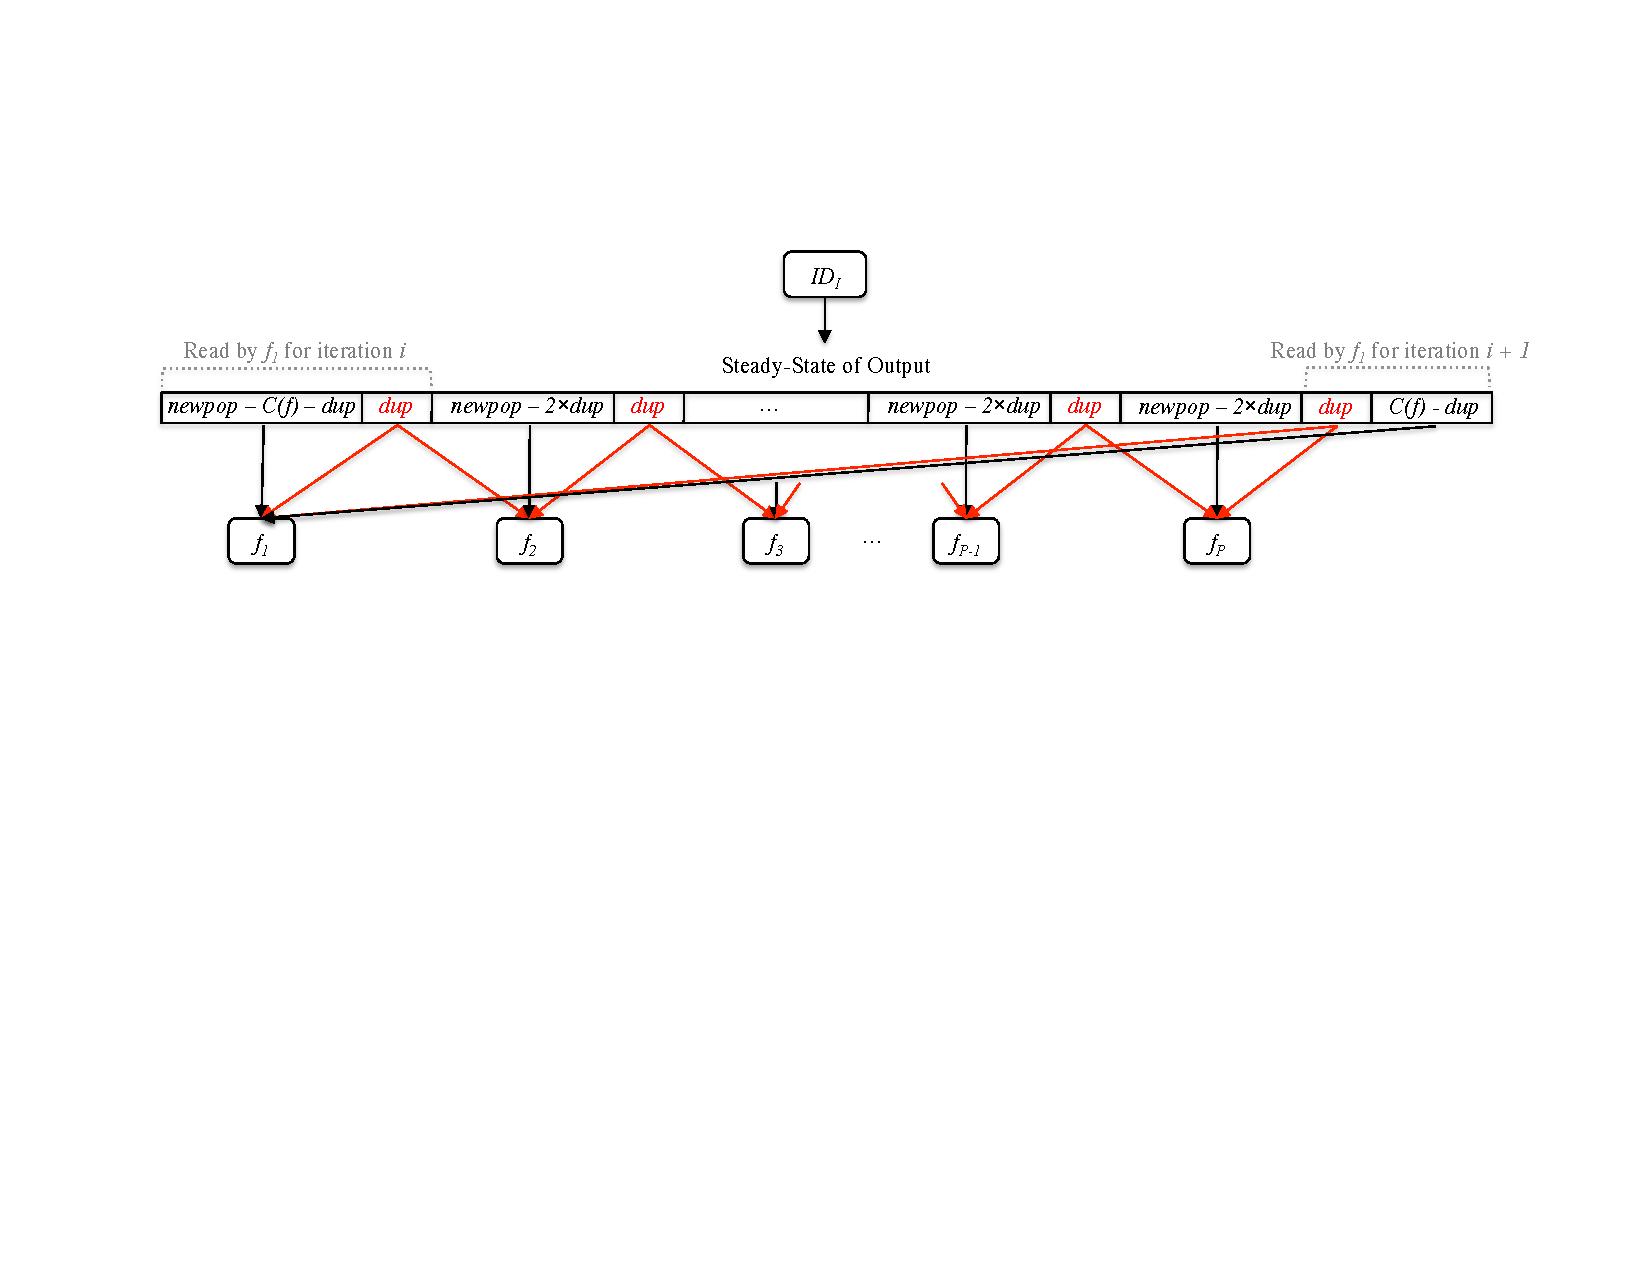
\includegraphics[width=6.3in]{figures/split-pattern.pdf}
\caption[The output distribution required for general
fission.]{
The steady-state output distribution installed for identity node
$ID_I$ by general fission.  Red edges denote items that are shared
across fission products via duplication. If $C(f) > dup$, $C(f) - dup$ items at the end of the
steady-state input are distributed to
$f_1$. \label{fig:split-pattern}}
\vspace{-10pt}
\end{figure*}

The general fission transformation creates two identity nodes ($ID_I$
and $ID_O$) that are encoded to implement the data distribution for
the fission products.  Figure~\ref{fig:split-pattern} illustrates the
pattern of communication between $ID_I$ and the products of $f$.  This
pattern is common to the transformation for all filters we seek to
fiss that meet the preconditions of the transformation.

The fission transformation has the following properties:
\begin{itemize}
\item No item is read by more than 2 fission products.
\item A fission product does not need to remember items across
  steady-state executions of itself. The peeking of the original
  filter $f$ is now encoded in the sharing across fission products
  achieved via the duplication pattern.
\item Only the first fission product $f_1$ is required to receive the $C(f)$
  initialization  items because $C(F) < (M(S,f) / p) \cdot o(W, f)$,
  and it will consume the $C(f)$ items on its first invocation.
\item The presence of the $C(f)$ items in the input buffer after
  initialization must be accounted for by shifting the read pattern
  for the fission products.  The first fission product $f_1$ is offset by
  $C(f)$ items in that it reads its first $C(f)$ items from the
  previous execution stage.  In the steady-state, $f_1$ executing at
  steady-state iteration $i$ shares items with $f_P$ executing at
  steady-state iteration $i-1$.
\item The computation and communication performed by $f$ during the
  initialization stage is transferred completely to the first fission
  product, $f_1$.  
% Since, by construction, only $f_1$ requires the
%   items remaining after the initialization stage.  The other fission
%   products are idle during this stage.
\end{itemize}

% The final steps of the general fission transformation applies
% \textsc{SynchRemove} to remove the identity filters, and stitch the
% communication directly between the fission products and $f$'s
% producer(s) and consumer(s).
 


% To understand the transformation, we first need to understand the item
% distribution and sharing that is required by fission on a filter $f$
% that adheres to the preconditions above.
% Figure~\ref{fig:fission-sharing2} gives another example of the input
% items required by fission products.  In this example, both:

% \[ C(f) = \mt{dup}_f < (M(S,f) / p) \cdot o(W, f) \]
% \[ M(S, f) \mod P = 0\]

% \noindent so $f$ adheres to the preconditions stipulated above for
% general fission.  In the example, the items read for $f$ plus its
% fission products for $P=4$ are shown for the initialization plus two
% steady-states.  After the initialization stage, $C(f) = 2$ items are
% enqueued to the input buffer by the producer(s) to $f$, and $M(S,f)
% \cdot o(W, f) = 16$ items are enqueued by the producer(s) for each
% steady-state.  Examining the sharing requirement for fission products of
% the second steady-state, we can see a pattern emerge with the following
% features:
%\section{Data Parallelization Common Case}

The techniques covered above are employed during the compiler flow
outlined in Chapter~\ref{ch:datapar} to effectively leverage data and
task parallelism.  The coarsened StreamIt graph is converted into a
general by employing \textsc{SynchRemove} (see
Section~\ref{sec:synch-remove} for details).  \textsc{JudiciousFission} is
performed on the coarsened general graph using the technique covered
in Section~\ref{sec:levels}.  Fission of a node in the general graph
replaces fission of a filter in the StreamIt graph (see
Section~\ref{sec:fission-streamit}) in the process of judicious
fission.  Conversion to the general graph with synchronization
removal, accompanied by employing general fission, greatly reduces the
inter-core communication requirement of the resulting mapping when
fissing filters that peek.  Figure~\ref{fig:fission-versus} gives a
simple example of the potential savings.

The design of the general fission algorithm was informed by the fact
that for most fission applications of judicious fission, a producer
and consumer are fissed by an equal width.  This is because in most of
our benchmarks, a level's width of task parallelism is equal to the
width of task parallelism for it's consuming level.  In this case,
fission on the general graph will map the bulk of communication to
intra-core resources.  Furthermore, in the next section we demonstrate
that the ratio of inter-core communication to total communication is
parametrizable for this case.

To understand why general fission achieves the reduction of inter-core
communication for this case, we must remember a few properties of the
steady-state schedule of the stream graph.  For single output producer
$f$ and single input consumer $g$, where $(f,g) \in E$:

\[ M(S, f) \cdot u(W, f) = M(S,g) \cdot o(W,g) \]

\noindent When $f$ and $g$ are fissed (employing general fission) by
the same amount $P$, the above equality no longer holds across all the
fission products if $g$ peeks.  This is because the peeking of $g$ is
converted into duplication of items to the products of $g$'s fission
application.  The fission products of $g$ each consumes more items
than each fission product of $f$ produces.  However, we can make it
the case that {\it most} of the outputs of a fission product $f_i$ are
directed to $g_i$, for each $1 \le i \le P$.  When each $f_i$ and
$g_i$ are mapped to the same core, the bulk of communication is
intra-core.

\begin{figure*}[t]
\centering
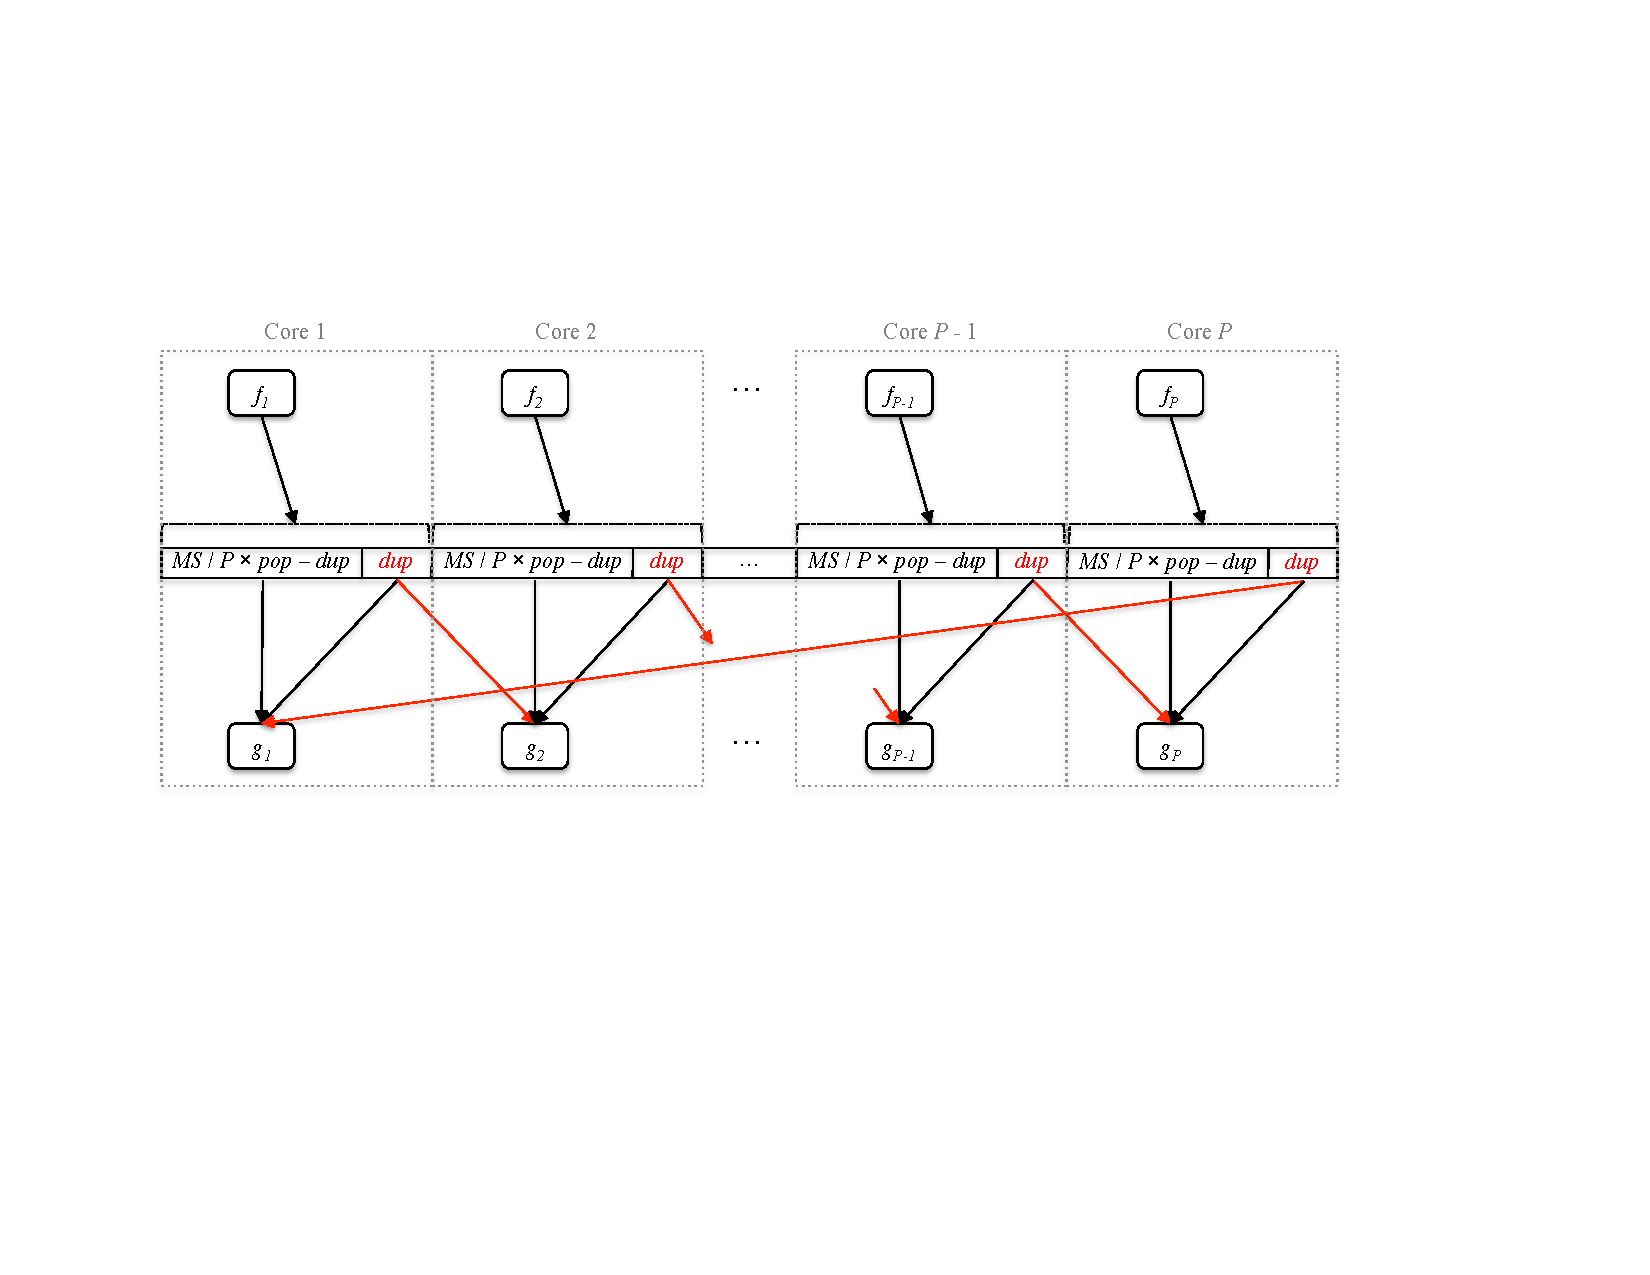
\includegraphics[width=6in]{figures/core-comm.pdf}
\caption[Communication between cores for fission of producer and
consumer.]{ Communication details for fission products of consumer $f$
  and producer $g$ each fissed by $P$.  $f$ was a single output node,
  and $g$ was a single input node.  Furthermore, $C(g) = \mt{dup}_g$.
  Each $f_i$, $g_i$ pair are mapped to the same core.
  The sizes of the buffer sections are in terms of $g$. Red arrows
  denote inter-core communication. \label{fig:core-comm}}
\end{figure*}

Figure~\ref{fig:core-comm} illustrates the details of communication
between $f$ and $g$ when each is fissed by $P$.  In the figure it is
assumed that $C(g) = \mt{dup}_g $, meaning the number of items
remaining after the initialization schedule equals the number of items
that $g$ inspected but did not pop.  Each $f_i$ produces $M(S,f)/p
\cdot u(S,f)$ items, while each $g_i$ must consume the original pop
rate multiplied by it's slice of $f$'s multiplicity plus the number of
inspected items of $g$:

\[ M(S,g)/P \cdot o(W, g) + C(g) \]

\noindent Since $M(S,g)/P \cdot o(W, g) = M(S,f)/p
\cdot u(S,f)$, the number of items each $f_i$ produces and the number
of items each $g_i$ consumes differs by $C(g)$.
As Figure~\ref{fig:core-comm} demonstrates, each $g_i$
receives $C(g)$ duplicated items from $g_{i-1}$ (with $g_1$
receiving from $f_p$).  When the fission products are assigned to
cores as given in the figure, the percentage of inter-core
communication to total communication can be reduced to:

\begin{equation}
\label{eq:min-dup}
\mt{InterCore}(g) = \frac{C(g)}{M(S,g) / P * o(W, g)}
\end{equation}

\noindent This percentage corresponds to the best case, in which a
producer and consume are fissed by the same amount and $C(g) =
\mt{dup}_g$.  This case is common in our benchmarks.

The next section covers a technique that seeks to decrease the percentage
of total communication that must be communicated inter-core.  The
technique directly decreases the number of items that are shared,
while also increasing the alignment of communication to minimize
inter-core communication.

%\section{Sharing Reduction}

A key design goal for the implementation of fission was that
communication between producers and consumers of the stream graph be
efficient.  Often when data parallelism is applied, the producer
filter is fissed at the same width as the consumer filter.  To make
this common case efficient, general graph fission communicates a large
number of items between disjoint producer-consumer pairs of products
of the fission.  Next, a small number of items (the number of items
inspected by the consumer filter) is duplicated and communicated from
producer to a consumer in a different pair.

\begin{figure*}[t]
\centering
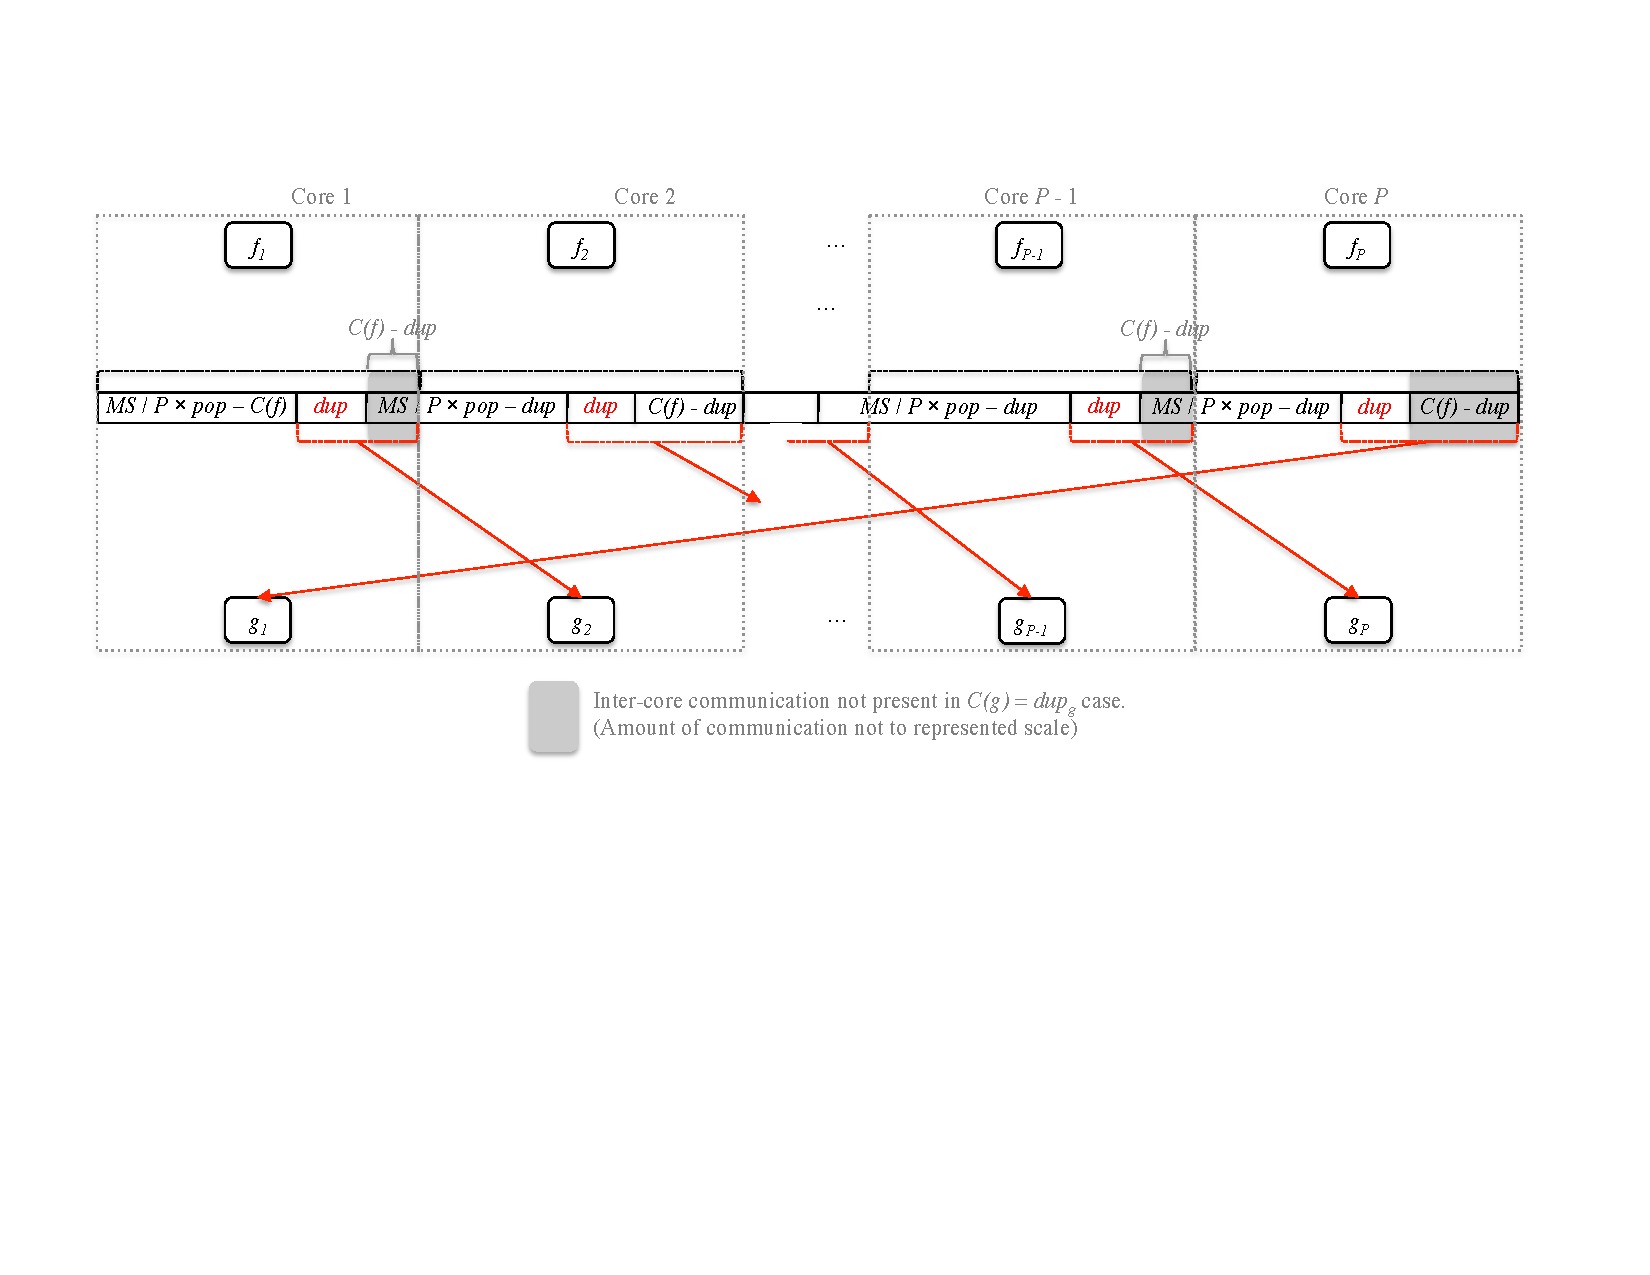
\includegraphics[width=6in]{figures/remaining-dup-case.pdf}
\caption[Extra inter-core communication when $C(g) > \mt{dup}_g$.]
{Inter-core communication details for fission products of consumer $f$
  and producer $g$ each fissed by $P$.  $f$ was a single output node,
  and $g$ was a single input node.  For $g$, $C(g) > \mt{dup}_g$.
  Each $f_i$, $g_i$ pair are mapped to the same core.  The sizes of
  the buffer sections are in terms of $g$. Red arrows denote
  inter-core communication.  \label{fig:remaining-dup}}
\end{figure*}

Figure~\ref{fig:remaining-dup} illustrates the details of
communication between $f$ and $g$ when each is fissed by $P$ with each
$f_i$ mapped to a distinct core, and to the same core as $g_i$.  From
the figure, notice that $C(g)$ items are communicated from $f_i$ to
$g_{i+ 1}$, with $f_P$ sending to $g_1$.  Of the $C(g)$ items,
$\mt{dup}_g$ items are required by both $g_i$ and $g_{i+1}$.  This
corresponds to the orignal number of input items of $g$ that were
inspected by not dequeued for one firing of $g$.  The remaining items,
$C(g) - \mt{dup}_g$, are required to be transfered from $f_i$ to
$g_{i+1}$ when $C(g) > \mt{dup}$ because of misalignment of the items
produced by $f_i$ and required by $g_i$.

When the fission products are assigned to
cores as given in the figure, the percentage of inter-core
communication to total communication can be quantified as:

\begin{equation}
%b\vspace{-2pt}
\label{eq:min-dup}
\mt{InterCore}(g) = \frac{C(g)}{M(S,g) / P * o(W, g)}
%\vspace{-4pt}
\end{equation}

\noindent This percentage corresponds to the case in which a
producer and consume are fissed by the same amount.  This case is
common in our benchmarks.

This section covers a technique that seeks to decrease the percentage
of total communication that must be communicated inter-core.  The
technique directly decreases the number of items that are shared,
while also increasing the alignment of communication to minimize
inter-core communication.

Since streaming applications typically execute for many iterations of
the steady-state, it is legal to increase the steady state by $c$.  As
long as this constant $c$ is less than the number of steady-state
iterations $I$ of the application, and $c$ is a factor of $I$.

By recognizing this property, we can directly reduce the amount of
inter-core communication that occurs between the fission products of a
fissed peeking filter for many cases of general fission, including the
common case.  In Equation~\ref{eq:min-dup} we can directly control the
steady-state multiplicity of $g$, $M(S,g)$.  We can calculate a
constant $c_g$ such that the percentage is less than a threshold
$T_{\mt{sharing}}$:

\begin{equation}
\label{eq:ic-thresh}
c_g = \frac{1}{T_{\mt{sharing}}} \cdot \frac{C(g) \cdot P}{M(S,g) \cdot o(W,g)}
\end{equation}

\noindent where $0.0 < T_{\mt{sharing}} \le
\mt{InterCore}$. Increasing the steady-state of the graph by $c_g$
before general fission is applied will assure that the percentage of
items duplicated will be equal to $T_{\mt{sharing}}$.  Sharing
reduction works by increasing the ratio of number of items that are
only needed by one product to the number of items that are needed by
two products.  When we increase the steady-state, in
Figure~\ref{fig:remaining-dup}, the shared (red) sections of the input
buffer to $g$ remain fixed in size, while the private sections of the
input buffer (black) grow.

\subsection{Sharing Reduction for Other Fission Cases}

The sharing reduction optimization does not apply as simply to all
cases of fission of a peeking filter.  Consider the case where we have
single output producer $f$ and single input consumer $g$ with $(f,g)
\in E$, but $f$ and $g$ are fissed by differing widths, i.e., $P_f \ne
P_g$.  This case engenders inter-core communication not only because
of sharing but because of the communication required by the differing
fission widths.  

Going forward, let us assume that $P_f > P_g$.  If $P_f$ is a multiple
of $P_g$, the analysis is straightforward: the percentage of
inter-core communication to total communication is $(1 -
\frac{P_g}{P_f}$). If $P_f$ is not a multiple of $P_g$ misalignment
also occurs because for one or more $g_j$, it's input does not begin
in alignment with any $f_i$'s.  The analysis of the percent of
inter-core communication for this latter case is complex, but it
suffices for our purposes to bound it by $(1 - \frac{P_g}{P_f})$.

Also consider the case where $g$ has multiple inputs. In this case $g$
receives $\mt{RI}(f, g, S) \cdot M(S, g) \cdot o(W,g)$ items from $f$
during the steady-state, and $(1 -\mt{RI}(f, g, S) \cdot M(S, g) \cdot
o(W,g))$ from its other producers. There is a choice: for which
producer of $g$ to optimize the communication of $g$? If $f$ is
chosen, then the assignment of filters to cores should minimize the
inter-core communication by co-locating the fission products of $f$
and $g$ just as the assignment would when $g$ is single input.
However, the calculation must now account for the inter-core
communication of the other producers sending to the fission products
of $g$. 

Now, considering both cases above, we define $\mt{InterCore}(g, f)$ to
approximate the percentage of inter-core communication to total
communication for the input of the fission products of $g$ optimizing
for the placement of the fission products of $f$:

\begin{equation}
\label{eq:tcomm-fopt}
 \mt{InterCore}(g, f)   =  (1 -\mt{RI}(f,g, S) \cdot \frac{P_g}{P_f})
 + \frac{P_g \cdot C(g)}{M(S, g) \cdot o(W, g)}
\end{equation}

\noindent The first term approximates the inter-core communication due
to the fission width discrepancy and the multiple inputs of $g$.  The
second term quantifies the percentage of inter-core communication
caused by the sharing due to peeking.

How do we decide whether it is worthwhile to apply the sharing
reduction optimization to $g$ given Equation~\ref{eq:tcomm-fopt}? When
the sharing reduction optimization is applied, the steady-state
multiplicity of $g$ is increased by a constant $c$.  If this is
applied to Equation~\ref{eq:tcomm-fopt}, the first term will be
unaffected, however the second term can be reduced because a smaller
percentage of steady-state items needs to be duplicated.  By Amdahl's
law, sharing reduction can only decrease $\mt{InterCore}(g,
f)$ to under $T_{\mt{sharing}}$ if the second term of Equation~\ref{eq:tcomm-fopt}
accounts for more than $(1-T_{\mt{sharing}} )$ of the duplication.  We
define a constant $T_{\mt{apply}}$ such that sharing
reduction should only be applied to $g$ optimizing for $f$ if:

\begin{equation}
\label{eq:apply-sharing}
T_{\mt{sharing}}  >  T_{\mt{apply}} \ge (1 -\mt{RI}(f,g, S) \cdot
\min(\frac{P_g}{P_f}, \frac{P_f}{P_g}))
\end{equation}

% \begin{equation}
% T_{\mt{sharing}}  >  T_{\mt{apply}} \ge (1 -\mt{RI}(f,g, S) \cdot
% \frac{P_g}{P_f})
% \end{equation}

\noindent Since it was first assumed that $P_f > P_g$, in order to
generalize we must choose the appropriate fraction of local
communication by taking the minimum of the two fission width ratios.

In the common case where $f$ and $g$ are fissed by the same width, and
$f$ has single output and $g$ has single input, the RHS of
Eq.~\ref{eq:apply-sharing} evaluates to 0, indicating to always apply
sharing reduction.  If however, the RHS of Eq.~\ref{eq:apply-sharing}
does not evaluate to 0, there exists inter-core communication that is
not attributed to sliding windows.  In this latter case,
$T_{\mt{apply}}$ determines at what percent of total inter-core
communication, non-sliding-window inter-core communication should
prevent the application of sharing reduction.  For example, if
$T_{\mt{apply}} = .05$, then we will apply sharing reduction only when
sliding window inter-core communication accounts or at least 95\% of
total inter-core communication for the proposed fission application of
$g$. $T_{\mt{apply}}$ prevents the application of sharing reduction to
fission when the bulk of inter-core communication of the fission is
not caused by sliding windows.

% For simplicity of analysis, let us assume that $C(g)
% = 0$, and $P_f$ is a multiple of $P_g$. Figure~\ref{fig:diff-widths}
% presents an example with these assumptions.  In the example, $f$ and
% $g$ are fissed by 8 and 4 respectively.  Since we want to maintain
% data parallelism, each $f_i$, $1 \le i \le P_f$, is mapped to a
% distinct core, as is each $g_j$, $1 \le j \le P_g$.  Since each $f_i$
% produces half the number of items required by each $g_j$, half the
% communication in this case is inter-core, caused by the misalignment
% of the rates of the producer and consumer fission products.


% Additionally, if $C(g) > 0$, it is required to share $C(g)$ items
% between two cores.  There are $P_g$ sections of $C(g)$ items, and this
% data has to be communicated inter-core to one other core.  Given this
% analysis, we can quantify an {\it approximation} of the percentage of
% inter-core communication for the fission application of $g$ when $P_f
% > P_g$:

% \begin{align}
% \mt{InterCore}(g) & = & \frac{(1 - \frac{P_g}{P_f}) \cdot M(S, g) \cdot o(W, g) +
% P_g \cdot C(g)}{M(S, g) \cdot o(W, g)} \\
% \label{eq:diff-fiss}
% \mt{InterCore}(g) & = & (1 - \frac{P_g}{P_f}) +
% \frac{P_g \cdot C(g)}{M(S, g) \cdot o(W, g)}
% \end{align}

% The first term on the RHS of Equation~\ref{eq:diff-fiss} gives the
% percentage of inter-core communication produced by the fission width
% inequality.  

% \begin{equation}
% \label{eq:tcomm-fopt1}
%  \mt{InterCore}(g,f)   = (1 - \mt{RI}(f,
%    g, S))  + (1 - \frac{P_g}{P_f}) \cdot \mt{RI}(f,
%    g, S)   + \frac{P_g \cdot C(g)}{M(S, g) \cdot o(W, g)} 
% \end{equation}

% \noindent The first term accounts for the percentage of items that $g$'s fission
% products receive from producers that are not products of $f$.  The
% second term, the percentage items that are communicated inter-core
% because of the fission width mis-alignment, must now account for the
% fact that not all items are from $f$.  Equation~\ref{eq:tcomm-fopt1}
% can be simplified to:


\subsection{Sharing Reduction Applied to the Stream Graph}
So far we have considered the application of the sharing reduction
optimization to a single filter $g$ in the stream graph.  Now we will
cover how to apply sharing reduction across all the filters of the
stream graph for which it is appropriate.  The goal is reduce the
percentage of inter-core communication due to the sharing between
fission products of all peeking filters to {\it approximately}
$T_{\mt{sharing}}$ of total inter-core communication for the fission
of all peeking filters.  Sharing reduction may not achieve
$T_{\mt{sharing}}$ because there may exist peeking filters that are to
be fissed for which Equation~\ref{eq:apply-sharing} cannot be
satisfied.  For these filters, we do not apply the sharing reduction
optimization.

The process of applying sharing reduction to the entire stream graph
consists of determining which filters are appropriate and determining
a steady-state multiplier by which to increase the graph.  To
determine the steady-state graph multiplier, the compiler calculates
the percentage of sharing over all of the filters which adhere to
Equation~\ref{eq:apply-sharing}.  Let $\Phi$ denote the set of filters
for which Equation~\ref{eq:apply-sharing} holds and that we seek to
fiss:

\begin{equation}
\label{eq:sr-mult}
c = \frac{1}{T_{\mt{sharing}}} \cdot \frac{\sum_{g \in \Phi} P_g \cdot C(g) }{\sum _{g \in
    \Phi} M(S, g) \cdot o(W, g)}
\end{equation}

\noindent Increasing the steady-state by $c$ for all filters of the
graph will reduce the total sharing for the filters of $\Phi$ to
$T_{\mt{sharing}}$.  




% In the
%  graph before fission is applied, $C(g)$ items will remain in the
%  input buffer of $g$ between steady-state iterations.  After fission by $P$,
%  for each steady-state, $g_1$ will first consume the $C(g)$ items that
%  $f_p$ sent it from the previous steady-state iteration.  $g_1$ will
%  then require:

% \[ M(S, g)/P \cdot o(W, g) + \mt{dup} - C(g)\]

% \noindent additional items from $f_1$.\footnote{It is guaranteed that
%   $M(S, g)/P \cdot o(W, g) > C(g)$ by the precondition of general
%   fission.} This requirement is less than the number of items that
% $f_1$ produces $M(S, g)/P \cdot o(W, g)$ since $C(g) > \mt{dup}$. So,
% $C(g) - \mt{dup}$ items must be transferred from $f_1$ to $g_2$ in
% addition to the shared and duplicated $\mt{dup}$. In all, $C(g)$ items
% must be transferred from $f_i$ to $g_{i+1}$.

%  Each $f_i$ produces $M(S,f)/p
% \cdot u(S,f)$ items, while each $g_i$ must consume the original pop
% rate multiplied by it's slice of $f$'s multiplicity plus the number of
% inspected items of $g$:

% \[ M(S,g)/P \cdot o(W, g) + C(g) \]

% \noindent Since $M(S,g)/P \cdot o(W, g) = M(S,f)/p
% \cdot u(S,f)$, the number of items each $f_i$ produces and the number
% of items each $g_i$ consumes differs by $C(g)$.
% As Figure~\ref{fig:core-comm} demonstrates, each $g_i$
% receives $C(g)$ duplicated items from $g_{i-1}$ (with $g_1$
% receiving from $f_p$).  

%\section{Data Parallelization of Stream Graph}
\label{sec:data-par}

General fission and sharing reduction are employed after
\textsc{JudiciousFission} (see Algorithm~\ref{alg:jd}) calculates a
fission width for each filter of the graph.  The formulation of
general fission in Section~\ref{sec:general-fission} includes two
preconditions for filter $g$:

\begin{equation}
\label{eq:fiss-precond1}
C(g) < (M(S,g) / P) \cdot o(W, g) 
\end{equation}
\begin{equation}
\label{eq:mod-fiss}
M(S,g) \mod P = 0
\end{equation}

\noindent The compiler is required to calculate a multiplication
factor $c$ for the entire graph that satisfies the preconditions for
every filter.  At the same time, $c$ applies sharing
reduction to the graph by increasing the graph such that
Equation~\ref{eq:sr-mult} is satisfied by the constant.

\textsc{DataParallelize} of Algorithm~\ref{alg:data-parallelize}
highlights the steps for data parallelizing the general graph
representation of the application.  This sequence is applied after the
StreamIt graph has been coarsened and converted to a general graph.
The algorithm first calculates the judicious fission widths for each
filter of the general graph.  For each peeking filter $g$ that will be
fissed, line~\ref{ln:dp1} finds the producer of $g$ that minimizes
Equation~\ref{eq:apply-sharing}.  If this value is below
$T_{\mt{apply}}$, $g$ is added to the sharing reduction calculation by
adding $g$'s shared items and $g$'s total items to the running totals
of each quantity.  Sharing reduction is incorporated into the
steady-state multiplier $\mt{minMult}$ in line~\ref{ln:dp2} employing
Equation~\ref{eq:sr-mult}.  The algorithm applies
Equation~\ref{eq:fiss-precond1} to each peeking filter that will be
fissed by maintain a running value of the minimum multiplier that
enforce the precondition (line~\ref{ln:dp3}).  The sharing reduction
multiplicity ($\mt{minMult}$) is required to be greater than the
precondition multiplier.  Because of the precondition of
Equation~\ref{eq:mod-fiss}, the final multiplication factor for
increasing the steady-state must be a multiple of all the fission
widths calculated by \textsc{JudiciousFission}.  The algorithm assures
this by finding the least common multiple of all the $P_f$'s greater
than $\mt{minMult}$ (line~\ref{ln:dp4}).  The steady-state
multiplicity of the graph is then increased by multiplying all of the
multiplicities by $c$.  Finally, each filter $f$ can be fissed by $P_f$ using
general fission.

\begin{algorithm}[th!]
\caption{Exploit Data Parallelism in the General Graph for $N$ Cores} \label {alg:data-parallelize}
\textsc{DataParallelize}($G = (V, E), N, T_{\mt{sharing}}, T_{\mt{apply}} $)
\begin{algorithmic}[1]
\State $\mt{preCondMult} \gets 1$, $\mt{sharingItems} \gets 0$, $\mt{totalItems} \gets 0$
\State $\triangleright$ For each filter in the graph find the fiss factor
\ForAll {$g \in V$}
\State $P_g \gets $ \Call{JudiciousFission}{$g$, $N$} 
\EndFor
\Statex
\State $\triangleright$ Calculate multiplier for fission preconditions and for sharing reduction
\ForAll {$g \in V$}
\State $\triangleright$ If this is a peeking filter we are fissing:
\If {$P_g > 1 \wedge C(g) > 0$}
\State $\triangleright$ Find the producer of $g$ with the lowest
value for Eq.~\ref{eq:apply-sharing}
\State $f \gets \min_{f \in \mt{In}(g)} (1 -\mt{RI}(f,g, S) \cdot
\min(\frac{P_g}{P_f},\frac{P_f}{P_g} )) $
\label{ln:dp1}
\State $\triangleright$ If the min value is below $T_{\mt{apply}}$,
then record the sharing and total communication
\If {$T_{\mt{apply}} \ge  (1 -\mt{RI}(f,g, S) \cdot
\min(\frac{P_g}{P_f},\frac{P_f}{P_g} ))$}
\State $\mt{sharingItems} \gets \mt{sharingItems} + P_g \cdot C(g)$
\State $\mt{totalItems} \gets \mt{totalItems} + M(S,g) \cdot o(W, g)$
\EndIf 
\State $\triangleright$ Assure that fissing peeking filters adhere to Eq.~\ref{eq:fiss-precond1}
\State $\mt{preCondMult} \gets \max(\mt{preContMult}, \frac{C(g) \cdot P_g}{M(S,g)
 \cdot o(W,g)})$  
\label{ln:dp3}
\EndIf
\EndFor
\Statex
\State $\triangleright$ Find the multiplier for sharing reduction
\State $\mt{minMult} \gets T_{\mt{sharing}} \cdot \frac{\mt{sharingItems}
}{\mt{totalItems}}$
\label{ln:dp2}
\State $\triangleright$ Make sure that multiplier assures all fissing peeking filters
adhere to  Eq.~\ref{eq:fiss-precond1}
\State $\mt{minMult} \gets \max(\mt{minMult}, \mt{preCondMult})$
\State $\triangleright$ Find the least common multiple of the $P_f$'s
greater than $\mt{minMult}$ to adhere to Eq.~\ref{eq:mod-fiss}
\State $c \gets $\Call{LCM}{$\forall P_f | f \in V$} $ >
\mt{minMult}$
\Statex
\label{ln:dp4}
\State $\triangleright$ Increase the steady-state by $c$
\ForAll {$f \in V$}
\State $M(S,f) \gets c \cdot M(S, f)$
\EndFor
\Statex
\State $\triangleright$ Apply general fission to all nodes in the graph
\ForAll {$f \in V$}
\State \Call{GeneralFiss}{$f$, $P_f$}
\EndFor
\end{algorithmic}
\vspace{10pt}
\end{algorithm}


Through empirical experimentation on FMRadio, Filterbank, and
ChannelVocoder, we have settled on $T_{\mt{sharing}} =.10$ and
$T_{\mt{apply}} = 0.05$. These constants are the sweet stop for the two
architectures employed in the experimentation, being a good compromise
between buffer size and inter-core communication.
Figure~\ref{fig:fm-gen-comm} demonstrates the efficiency of general
fission for the FMRadio benchmark when judiciously fissed to 4 cores.
In the example, the coarsened version of FMRadio is given on the left.
The steady-state of FMRadio is increased by 2560 so that the total
sharing is under 10\%.  The last filter in the graph, the
$\mt{Equalizer}$ has a large $\mt{dup}$, and this had to be overcome
for each core.


%\section{Experimental Evaluation}

In this section we present an evaluation of the contributions of this
paper and compare to previous techniques for compiling stream programs
to multicore architectures.  This section will include an elaboration
of the following contributions and conclusions:

\begin{itemize}
\item Our technique for exploiting coarse-grained data parallelism
produces abundant parallelism and achieve a geometric mean performance
gain of 9.9x over a strictly task parallel baseline.
\item Coarse-grained software pipelining is a
an effective technique for extracting parallelism beyond task and data
parallelism, with an additional geometric mean speedup of 1.45x. On
its own, our software pipelining technique affords a 7.7x performance
gain over a task parallel baseline.
\item The combination of the techniques presented in this paper
improves upon previous work that exploited a combination of task and
pipeline parallelism.
\end{itemize}

First, we present a description of the benchmark suite employed
in the evaluation.

\begin{figure*}[t]
\centering
\psfig{figure=benchchar.eps, width=6.5in}
\caption{Benchmark characteristics
\protect\label{fig:benchchar}}
\end{figure*}

\subsection{Benchmark Suite}
We evaluate our techniques using the benchmark suite given in Figure
\ref{fig:benchchar}.   The benchmark suite consists of 12 StreamIt
applications. MPEG2Decoder implements the block decoding and the
motion vector decoding of an MPEG-2 decoder, containing approximately
one-third of the computation of the entire MPEG-2 decoder.  Also, the
DCT benchmark implements a 16x16 IEEE reference DCT while the
MPEG2Decoder benchmark includes an 8x8 IEEE fast DCT as a component.
For additional information for MPEG2Decoder, Vocoder, and Radar,
please refer to \cite{ipdps2006},
\cite{seneff80}, and \cite{pca}, respectively. 

In the table, the measurements given in each column are obtained from
the stream graph graph as conceived by the programmer, before it is
transformed by our techniques.  The ``Filters'' columns gives the
total number of filters in the stream (including file input filters
and file output filters that are not mapped to cores).  The number of
filters that perform peeking is important because peeking filters
cannot be fused without introducing shared state.  Thus, once a
peeking filter is fused, it cannot be fissed. In the table, the column
labeled ``Shortest Path'' and ``Longest Path'' give the shortest path
and the longest, path from source to sink. ``Comp / Comm'' gives the
static estimate of the computation to communication ratio of each
benchmark for one steady-state execution. This is calculated by
totaling the computation estimates across all filters and dividing by
the number of items communicated per steady-state. Notice that
although the computation to communication ratio is high across our
benchmarks, we demonstrate that inter-core synchronization is an
important factor to consider.

The benchmarks are sorted in ascending order of the final column,
``Stateful work''. This is percentage of the statically estimated work
performed per steady-state by all filters that have state divided by
the total work performed by all filters per steady-state.  Referring
to Figure \ref{fig:benchchar}, we see that three of our benchmarks
include stateful computation.  The stateful computation performed in
MPEGDecoder is insignificant and expressed as...
\textbf{Bill, can you talk about the statefull computation in
MPEG, radar, and vocoder}.


\begin{figure*}[t]
\centering
\psfig{figure=maingraph.eps, width=6.5in}
\caption{Task, Task + Data, and Task + Data + Software Pipeline
\protect\label{fig:main_comp}}
\end{figure*}

\subsection{Exploiting Coarse-Grained Data Parallelism}
To motivate the necessity of our parallelism extraction techniques let
us first consider the task parallel execution model.  This model
closely approximates a thread model of execution where the only form
of coarse-grained parallelism exploited is fork/join parallelism.  In
our implementation, the sole form of parallelism exploited in this
technique is the parallelism across the children of a splitjoin. The
first bar of Figure \ref{fig:main_comp} gives the throughput speedup
of the each of our benchmarks running in the task parallel model
executing on 16-core Raw normalized to sequential StreamIt executing
on a single core of Raw.  For the remainder of the presentation,
unless otherwise noted, we target all 16 cores of Raw.  The geometric
mean performance speedup for task parallel is 2.27x over sequential
performance. We can see that for most of our benchmarks, little
parallelism is exploited, notable exceptions are Radar,
ChannelVocoder, and FilterBank.  Each contains wide splitjoins of
load-balanced children.  In the case of BitonicSort, the task
parallelism is expressed at too fine a granularity for the
communication system.  Given that we are targetting a 16-core
processor, a mean speedup of 2.27x is inadequate.

The StreamIt programming model facilitates relatively simple analysis
to determine opportunities for data parallelism.  But the granularity
of the transformations must account for the additional synchronization
incurred by data-parallelizing a filter.  If we attempt to exploit
data-parallelism a fine granularity, by simply replicating each
stateless filter across the cores of the architecture we run the risk
of overwhelming the communication substrate of the target
architecture.  To study this, we implemented a simple algorithm for
data parallelism, replicate each filter by the number of cores,
mapping each to its own core.  In
\ref{fig:fine-dup}, we show this technique normalized to single-core
performance.  \textbf{todo!}

The second bar of Figure \ref{fig:main_comp} gives the speedup of
coarse-grained data parallelism over single-core StreamIt. The mean
speedup across our suite is 9.9x over single-core and 4.36x over our
task parallel baseline (not shown in the figure).  BitonicSort, whose
original granularity was too fine, now achieves a 8.4x speedup over a
single-core. 6 of our 12 applications are stateless and non-peeking,
and thus fuse to one filter that is fissed 16 ways.  For these
benchmarks the mean speedup is 11.1x over the single-core.  For DCT,
the algorithm data-parallelizes the bottleneck of the application (a
single filter that performs more than 6x the work of each of the other
filters).  For DCT, coarse-grained data parallelism achieves a 14.6x
speedup over single-core, while fine-grained achieves only 4.0x
because it fisses at too fine a granularity, improperly considering
synchronization.  Coarsening and then parallelizing reduces the
synchronization costs of data parallelizing.  For Radar and Vocoder,
data parallelism is paralyzed by the preponderance of stateful
computation.

\subsection{Exploiting Coarse-Grained Software Pipeline Parallelism}

\begin{figure}[t]
\centering
\psfig{figure=softpipe_graph.eps, width=3.2in}
\caption{Task and Task + Software Pipeline
\protect\label{fig:softpipe_graph}}
\end{figure}
Our novel technique for coarse-grained software pipelining is
effective for exploiting coarse-grained parallelization (though it
under-performs when compared to coarse-grained data parallelism).
More importantly, combining software pipelining with our data
parallelism techniques, provides a cumulative performance gain,
most especially for applications with stateful computation.

Figure \ref{softpipe_graph} considers coarse-grained software
pipelining and task parallelism normalized to single-core performance.
On average, software pipelining has a speedup of 7.7x over single-core
(compare to 9.9 for data parallelism) and a speedup of 3.4x over task
parallelism. Software pipelining performs well when it can effectively
load-balance the packing of the dependence-free steady-state.  In the
case, of Radar, TDE, FilterBank, and FFT, software pipelining achieves
comparable or better performance compared to data parallelism (see
Figure \ref{fig:thruput}).  For these applications, the workload is
not dominated by a single filter and the resultant schedules are
statically load-balanced across cores.  For the Radar application,
software pipelining achieves a 2.3x speedup over data parallelism and
task parallelism because there is little coarse-grained data
parallelism to exploit and it can more effectively schedule the
dependence-free steady-state.

However, when compared to data parallelism, software pipelining is
hampered by its inability to reduce the critical path when the
critical path contains stateless work (e.g., DCT, MPEGDecoder).  Also,
our data parallelism techniques tend to coarsen the stream graph more
than Selective Fusion, removing more synchronization.  For example, in
DES, the Selective Fusion Algorithm makes a greedy decision that it
cannot remove communication affecting the critical path workload.
Software pipelining performs poorly for this application when compared
to data parallelism, 6.9x versus 13.9x over single core, although it
calculates a load-balanced mapping.  Another consideration when
comparing software pipelining to data parallelism is that the software
pipelining techniques rely more heavily on the accuracy of the static
work estimation strategy, although it is difficult to quantify this
effect.

When we software pipeline the data-parallelized stream graph, we
achieve a 45\% mean speedup over data parallelism alone. The
cumulative effect is most prominent when the application in question
contains significant amounts of stateful computation.  For example,
the combined technique achieves a 69\% speedup over each individual
technique for Vocoder. For most of our other applications, software
pipeline further coarsens the stream graph without affecting the
critical path work (as estimated statically) and performs inter-core
communication in parallel.  Each reduces the synchronization
encountered on the critical path.

The combined technique depresses the performance of MPEG by 6\%
because the Selective Fusion component of the software pipeliner fuses
one step too far.  In most circumstances, fusion will help to reduce
inter-core synchronization by using the local memory of the core for
buffering. Consequently, the algorithm does not model the
communication costs of each fusion step. In the case of MPEG, it fuses
too far and adds synchronization by fusing two elements of a splitjoin
that perform little work.  The combined filter communicates more data
across the splitjoin than its sibling (who perform much more work).
The critical path of the application is increased because the
synchronization cost of splitting and joining increases.  The combined
technique also hurts Radar as compared to only software pipelining
because we fiss too aggressively and create synchronization across the
critical path.

In Figure \ref{fig:thruput}, we report the compute utilization and the
MFLOPS performance for each benchmark employing the combination of our
techniques. Note that for our target architecture, the maximum number
of MFLOPS achievable is 7200.  The compute utilization is calculated
as the number of instructions issued on each computer processor
divided by the total number possible for a steady-state.  The
utilization accurately models pipeline hazards and stalls of Raw's
single issue, in-order processing cores.  We achieve generally
excellent compute utilization; in 7 cases the utilization is 60\% or
greater.


\subsection{Comparison To Previous Work}

\begin{figure}[t]
\centering
\psfig{figure=vs_space_graph.eps, width=3.2in}
\caption{Task + Pipeline and Task + Data + Software Pipeline
\protect\label{fig:vs-space}}
\end{figure}

\begin{figure*}[t]
\centering
\psfig{figure=thruput.eps, width=6.5in}
\caption{Comparison and Task + Data + Software Pipeline Performance Results
\protect\label{fig:thruput}}
\end{figure*}
In Figure \rev{fig:vs-space} we show our combined technique normalized
to our previous work \cite{streamit-asplos}.  

Space good versus us for applications composed of long pipelines with little
splitting, including FFT5, tde

Serpent is fused down to a load-balanced pipeline, splitjoins
composed in a pipeline, space version has util of 64\% we are fusing
then taking advantage of pipeline parallelism, not always the right
thing to do.

Talk more about using on-chip network

Also the way we simulate input differs between the two backends.  Task
+ Pipeline attaches the input and output devices to the chip in the
place of dram, and the input is continuously streamed onto the chip.
The new backend fetches input and writes output from/to the DRAMs,
generating a DRAM command.

Raw's on-chip network is well-suited to pipeline communication, but it
does not approximate any other multicore.

DCT: must be partitioned to 16 tiles, the bottleneck is fissed 2 ways,
but the remaining stages must be fused to 4-way and they become the
bottleneck, plus synchronization!

MPEG: space partitioner must fuse down to 16 tiles removing task
parallelism of the program, and the work is not evenly distributed
across the application, resulting partitioning is not load-balanced,
dominated by a single filter that does more than 2x the amount of work
than the next largest filter.

DES:somewhat complicated graph repeated 4 time between some filters,
space partitioner is forced to partition these 4 containers (8 filters
each) into 2 filters that are not load balanced.  Synchronization
issues not alleviated when forced to fuse to pipeline.

Stateful benchmarks, compare without softpipe to space, and
then softpipe kicks in, hopefully, like 
vocoder:
beamformer:Task + Data loses to space by 19\%, T+D+SP beats space by
38\%
vocoder:T+D loses to space by 18\%, T+D+SP beats space by 30\%.


\section{Related Work}
\label{sec:related}

These capabilities enable a programmer to write an application and its
filters at a natural granularity that is independent of
parallelization considerations enabling portable, reusable, and
malleable code.  Furthermore, fine-grained implementations of filters
enables the compiler to perform guided filter fusion that balances
data and instruction cache behavior~\cite{sermulins-lctes05}.


Need to address the coarsening issue.  Brook, which disallows state
would force the user to just coarsen the filter.  Why wouldn't someone
just coarsen?  


\section{Conclusions and Future Work}
\label{sec:conclusion}

This paper makes two contributions.  First, it introduces teleport
messaging: a powerful language construct enabling precise message
delivery between nodes of a distributed stream program.  In comparison
with other methods to implement messaging functionality in a
Synchronous Dataflow (SDF) model, teleport messaging is arguably more
readable, more robust, and easier to maintain.  In addition, our
implementation of teleport messaging in the StreamIt compiler resulted
in a 49\% performance improvement for a frequency hopping radio
running on a cluster of workstations.  Like several declarative
language constructs, teleport messaging improves performance by
exposing the true dependences to the compiler and allowing it to
optimize the communication.

%% We outlined several possible applications of $\sdep$, including
%% latency constraints, debugging, speculation, and program analysis, and
%% we look forward to pursuing these directions in the future.

Second, this paper formulates $\sdep$, a natural and useful dependence
representation for the streaming domain.  While this paper applies
$\sdep$ to a new language construct, we envision other applications as
well.  For example, $\sdep$ could be used in a debugger to identify
which iterations of an upstream actor are affecting a given iteration
of a downstream actor.  In a software-based speculation
system~\cite{frank-thesis}, $\sdep$ could be applied to trace the
effects of a failed prediction and to roll back the appropriate actor
executions.  $\sdep$ also offers a new method for measuring latency in
a stream graph.  Similar to representations such as dependence
levels~~\cite{AK82}, direction vectors~\cite{wolfe82}, and dependence
polyhedra~\cite{Irig88} for scientific programs, $\sdep$ provides
dependence information that could be used to test or verify program
transformations.

There are some limitations in the current study that are fertile
grounds for future research.  First, our formulation of $\sdep$
requires a directed path in the stream graph (aligned with the
direction of data flow) between the actors in question.  We are
generalizing $\sdep$ to actors that run in parallel by leveraging
their data dependences with common predecessors (upstream) or
successors (downstream).  Second, as detailed in
Section~\ref{sec:constraints}, we do not solve the general scheduling
problem that incorporates overlapping constraints from teleport
messaging; even determining whether or not a set of constraints is
feasible (especially during the initialization
schedule~\cite{karczma-thesis}) seems to be an interesting question.
Third, in the current model only actors can send and receive messages.
We are extending this into a hierarchical model where stream
containers (such as pipelines) can also receive events and dispatch
them precisely to other streams.  Finally, our approach relies on the
static communication rates present in SDF.  It would be interesting to
consider teleport messaging in a more dynamic context; for example,
downstream non-negative latency messages could be immediately
supported by embedding messages in data items, while other messages
might require speculative delivery or modified timing contracts.

Our work can be viewed as the integration of dynamic behavior into a
static dataflow language.  Our insight is that there is a class of
control messages that only adjust a parameter in the target actor;
they do not otherwise affect the input or output channels upon
delivery.  This model enables a hybrid scheduling scheme in which the
steady-state dataflow is exactly orchestrated at compile time, but
there are windows in which a message could adjust an internal field of
an actor between its execution steps.  We consider this to be a
promising avenue for creating a unified development environment that
captures all aspects of stream application development without
sacrificing either performance or programmability.


% \acks
% Acknowledgments, if needed.

% We recommend abbrvnat bibliography style.
\footnotesize
\bibliography{references}
\bibliographystyle{IEEEtran}

\clearpage
%\appendix
%\begin{figure*}
%\centering
%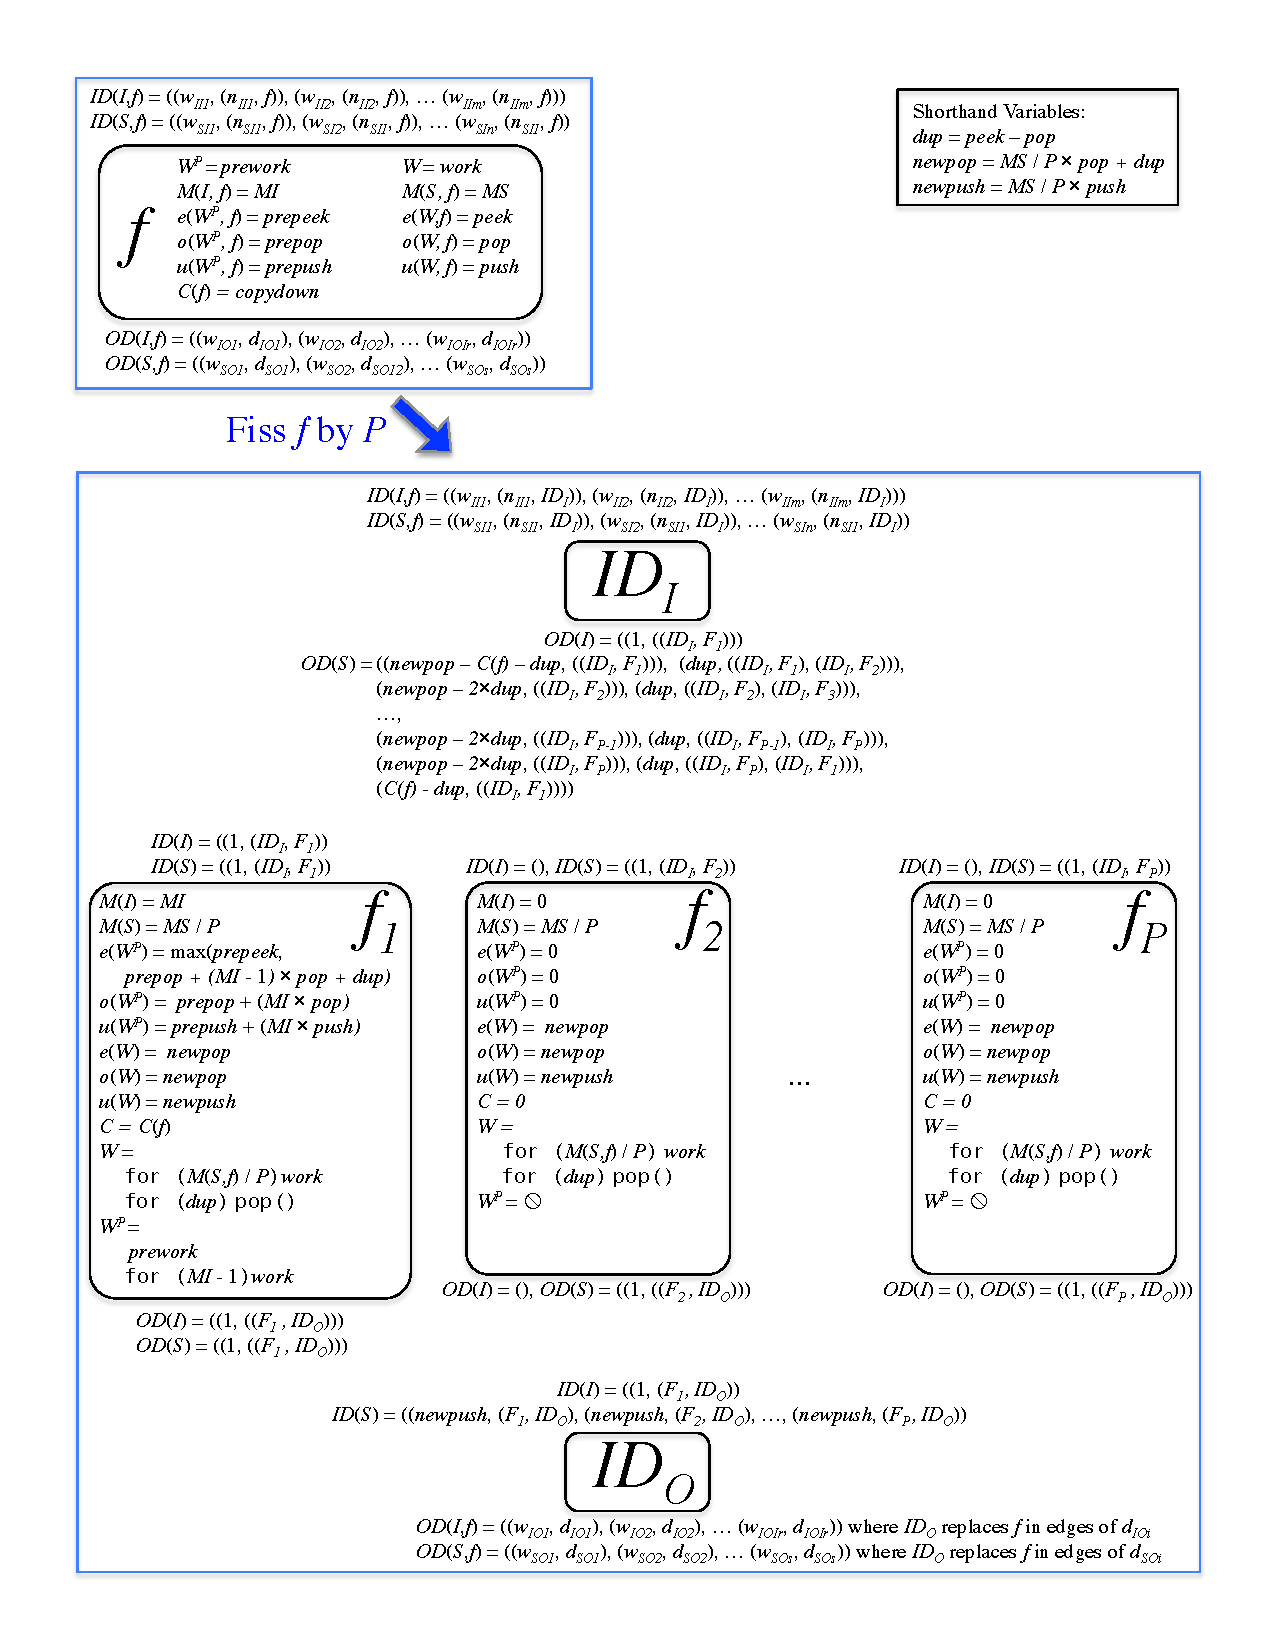
\includegraphics[width=\textwidth]{figures/general-fission.pdf}
%\caption[Fission of a node in the general stream graph.]{Appendix: Fission of a
%  node $f$ by $P$ in the general stream
%  graph.\label{fig:general-fission}}
%\end{figure*}


\end{document}

